% This is samplepaper.tex, a sample chapter demonstrating the
% LLNCS macro package for Springer Computer Science proceedings;
% Version 2.21 of 2022/01/12
%
\documentclass[runningheads]{llncs}
%
\usepackage[T1]{fontenc}
% T1 fonts will be used to generate the final print and online PDFs,
% so please use T1 fonts in your manuscript whenever possible.
% Other font encondings may result in incorrect characters.
%
\usepackage[utf8]{inputenc}
\usepackage[english]{babel}
\usepackage{booktabs}
\usepackage{hyperref}
\usepackage[utf8]{inputenc}
\usepackage[english]{babel}
\usepackage{booktabs}
\usepackage{hyperref}
\usepackage{graphicx}
% Used for displaying a sample figure. If possible, figure files should
% be included in EPS format.
%
\usepackage[vlined,algoruled,linesnumbered]{algorithm2e}
\usepackage{amsmath,amssymb,nccmath,mathtools}
\usepackage{tabularx}
\usepackage{siunitx}
\usepackage[vlined,algoruled,linesnumbered]{algorithm2e}
\usepackage{amsmath,amssymb,nccmath,mathtools}
\usepackage{tabularx}
\usepackage{siunitx}
% If you use the hyperref package, please uncomment the following two lines
% to display URLs in blue roman font according to Springer's eBook style:
\usepackage{xcolor}
\renewcommand\UrlFont{\color{blue}\rmfamily}
\urlstyle{rm}
%
%
%
\usepackage{array,multirow,makecell}
\setcellgapes{1pt}
\makegapedcells
\newcolumntype{R}[1]{>{\raggedleft\arraybackslash }b{#1}}
\newcolumntype{L}[1]{>{\raggedright\arraybackslash }b{#1}}
\newcolumntype{C}[1]{>{\centering\arraybackslash }b{#1}}
\usepackage{stmaryrd}

\SetKwRepeat{Do}{do}{while}%

\usepackage{enumerate}
%
%
\begin{document}
%
\title{Masked Computation of the Floor Function and Its Application to the FALCON Signature}
%
\titlerunning{Masked Floor Function For FALCON}
% If the paper title is too long for the running head, you can set
% an abbreviated paper title here
%
\author{Justine Paillet\inst{1,3}\orcidID{0009-0009-6056-7766} \and
  Pierre-Augustin Berthet\inst{2,3}\orcidID{0009-0005-5065-2730} \and
C\'edric Tavernier\inst{3}\orcidID{0009-0007-5224-492X}}
%
\authorrunning{J Paillet et al.}
% First names are abbreviated in the running head.
% If there are more than two authors, 'et al.' is used.
%
\institute{
  Université Jean-Monnet, Saint-\'Etienne, France, \email{justine.paillet@univ-st-etienne.fr}
  \and
  Télécom Paris, Palaiseau, France, \email{berthet@telecom-paris.fr}
  \and
  Hensoldt SAS FRANCE, Plaisir, France, \email{<pierre-augustin.berthet,justine.paillet,cedric.tavernier>@hensoldt.net}
}
%
\maketitle              % typeset the header of the contribution
%
\begin{abstract}
With the ongoing standardization of new Post Quantum Cryptography (PQC) primitives by the National Institute of Standards and Technology (NIST), it is important to investigate the robustness of new designs to Side Channel Analysis (SCA). Amongst those future standards is Falcon, a lattice-based signature which relies of rational numbers. It thus requires an implementation using floating point arithmetic, which is harder to design well and secure. While recent work proposed a solution to mask the addition and the multiplication, some roadblocks remains, most noticeably how to protect the floor function. In this work we propose several methods to protect the computation of the floor function. We provide mathematical proofs of our methods as well as formal security proof in the probing model using the Non-Interference concepts. We also discuss their application to the FALCON Signature.
With the ongoing standardization of new Post Quantum Cryptography (PQC) primitives by the National Institute of Standards and Technology (NIST), it is important to investigate the robustness of new designs to Side Channel Analysis (SCA). Amongst those future standards is Falcon, a lattice-based signature which relies of rational numbers. It thus requires an implementation using floating point arithmetic, which is harder to design well and secure. While recent work proposed a solution to mask the addition and the multiplication, some roadblocks remains, most noticeably how to protect the floor function. In this work we propose several methods to protect the computation of the floor function. We provide mathematical proofs of our methods as well as formal security proof in the probing model using the Non-Interference concepts. We also discuss their application to the FALCON Signature.

\keywords{Floor Function \and Floating-Point Arithmetic \and Post-Quantum Cryptography \and FALCON \and Side-Channel Analysis \and Masking}
\end{abstract}
%
%
%
\section{Introduction}
With the rise of quantum computing, mathematical problems which were hard to solve with current technologies will be easier to breach. Amongst the concerned problem is the Discrete Logarithm Problem (DLP) which can be solved in polynomial times by the Shor quantum algorithm \cite{doi:10.1137/S0036144598347011}. As much of the current asymmetric primitives rely on this problem and will be breach, new cryptographic primitves are studied. The National Institute of Standards and Technology (NIST) launched a post-quantum standardization process \cite{chen2016report}. The finalists are CRYSTALS Kyber \cite{8406610,nistfips203mlkem}, CRYSTALS Dilithium \cite{Ducas_Kiltz_Lepoint_Lyubashevsky_Schwabe_Seiler_Stehlé_2018,nistfips204mldsa}, SPHINCS+ \cite{10.1145/3319535.3363229,nistfips205shdsa} and FALCON \cite{prest2020falcon}.

\medskip

\noindent Another concern for the security of cryptographic primitives is their robustness to a Side-Channel opponent. Side-Channel Analysis (SCA) was first introduced by Paul Kocher \cite{10.1007/3-540-68697-5_9} in the mid-1990. This new branch of cryptanalysis focuses on studying the impact of a cryptosystem on its surroundings. AS computations take time and energy, an opponent able of accessing the variation of one or both could find correlations between its physical observations and the data manipulated, thus resulting in a leakage and a security breach. Thus, the study of weaknesses in implementations of new primitives and the ways to protect them is an active field of research.

\medskip 

\noindent While they have been many works focusing on CRYSTALS Dilithium and CRYSTALS Kyber, summed up by Ravi et al. \cite{10.1145/3603170}, FALCON is noticeably harder to protect. Indeed, the algorithm relies on floating-point arithmetic, for which there is little litterature on how to protect it.
%
\subsubsection{Related Work} Previous works have identified two main weaknesses within the signing process of Falcon : the pre-image computation and the Gaussian sampler. The pre-image computation was proved vulnerable by Karabulut and Aysu \cite{9586131} using an ElectroMagnetic (EM) attack. Their work was later improved by Guerreau et al. \cite{Guerreau_Martinelli_Ricosset_Rossi_2022}. To counter those attacks, Chen and Chen \cite{Chen_Chen_2024} propose a masked implementation of the addition and multiplication of FALCON. However, they did not delved into the second weakness of Falcon, the Gaussian sampler.\newline
The Gaussian sampler is vulnerable to timing attacks, as shown by previous work \cite{10.1007/978-3-662-53140-2_16,10.1145/3133956.3134028,cryptoeprint:2019/478,10.1145/3133956.3134023}. A isochronous design was proposed by Howe et al. \cite{10.1007/978-3-030-44223-1_4}. However, a successful single power analysis (SPA) was proposed by Guerreau et al. \cite{Guerreau_Martinelli_Ricosset_Rossi_2022} and further improved by Zhang et al. \cite{10.1007/978-3-031-30634-1_19}. There is currently no masking countermeasure for FALCON's Gaussian Sampler. Existing work \cite{10.1007/978-3-031-07082-2_9} tends to re-write the Gaussian Sampler to remove the use of floating arithmetic, thus avoiding the challenge of masking the floor function. 
%
\subsubsection{Our Contribution}
In this work we further expand the countermeasure from Chen and Chen \cite{Chen_Chen_2024} and apply it to the Gaussian Sampler. We propose a masking method based on the mantissa truncation to compute the floor function. We also propose a generic method to arithmetize the computation of the floor function. We discuss the application of both methods to masking FALCON.

\medskip

Relying on the previous work of Chen and Chen \cite{Chen_Chen_2024}, we also verify the higher-order security of our method in the probing model. Our formal proofs rely on the Non-Interference (NI) security model first introduced by Barthe et al. \cite{10.1145/2976749.2978427}.

\medskip

Finally, we provide some performances of our methods and compare them with the reference unmasked implementation and the previous work of Chen and Chen \cite{Chen_Chen_2024}. The implementation is tested on a personal computer with an Intel-Core i7-11850H CPU.
%
\section{Notation and Background}\label{sec:background}
\subsection{Notation}
\begin{itemize}
  \item We denote by $\mathbb{R}\backsim \mathbb{Z}$ any real number which is not an integer. For $x\in\mathbb{R}$, we denote the floor function of $x$ by $\lfloor x \rfloor$.
  \item We will use the dot $.$ as the separator between the integer part $i$ and the fractional part $f$ of a real number $x=i.f$.
  \item We denote the floor function of $x$ with $n$ decimals of absolute precision by $\lfloor x \rfloor_n$. Absolute precision implies $\lfloor x\rfloor_n = \lfloor x \rfloor + 0.\{0\}^n\|[0;9]^*$. This also implies that $0 \leq \lfloor x \rfloor_n - \lfloor x \rfloor < 1\times 10^{-n}$.
  \item We denote the floor function of $x$ with $n$ decimals of relative precision $\alpha\in[\num{0.1};1)$ by $\lfloor x \rfloor_n^\alpha$. Relative precision implies $-\alpha\times 10^{-n} < \lfloor x \rfloor_n^\alpha - \lfloor x \rfloor < \alpha\times 10^{-n}$.
  \item Let $a,b\in\mathbb{R}^2$. Let $k\in\mathbb{N}$. We say that $a\equiv_k b$ if $\lfloor a\rfloor = \lfloor b \rfloor$ and they have the same number of $0$ at least for the first $k$ decimals: $\lfloor a \rfloor + 0.\{0\}^k\|[0;9]^*$. For instance, $\num{4.05} \equiv_k \num{4.09}$ at precisions $k=0$ and $k=1$ but not at precision $k=2$.
  \item If $(b_i)$ is a 1-bit Boolean shares for value b, we denote $(-b_i)$ as the 64-bit Boolean shares for $2^{64} - b$. It means that if $b=0$, $(-b_i)$ is a 64-bit boolean shares for $0$, and
  $b=1$, $(-b_i)$ is a 64-bit boolean shares for 0x\textsc{ffffffffffffffff}. 

  
\end{itemize}
% 
\subsection{FALCON Sign}
FALCON \cite{prest2020falcon} is a Lattice-Based signature using the GPV framework over the NTRU problem. In this paper we will focus on the Gaussian Sampler used in the signature algorithm. For more details on the key generation or the verification, please refer to the reference paper \cite{prest2020falcon}.

\subsubsection{Signature} The signature follows the Hash-Then-Sign strategy. The message $m$ is salted with a random value $r$ and then hashed into a challenge $c$. The remainder of the signature aims at building an instance of the SIS problem upon $c$ and a public key $h$, \emph{id est} finding $\vec{s} =(s_1,s_2)$ such as $s_1 + s_2 h = c$. To do so, the need to compute $\vec{s} = (\vec{t}-\vec{z})\mathbf{B}$, with $\vec{t}$ a pre-image vector and $\vec{z}$ provided by a Gaussian Sampler. Chen and Chen \cite{Chen_Chen_2024} focuses on masking the pre-image vector computation. In this work we intend to mask the Gaussian Sampler. The signature algorithm is detailled in Algorithm \ref{alg:falconsign}:

\begin{algorithm}[H]
  \caption{FALCON Sign \cite{prest2020falcon}}
  \label{alg:falconsign}
\end{algorithm}

\subsubsection{Gaussian Sampler}

\paragraph{ApproxExp.} This function return $2^{63}\times ccs \times e^{-x}$.

C =
$ \left[\begin{array}{cc}
     \textsc{0x00000004741183a3}, & \textsc{0x00000036548cfc06},\\
        \textsc{0x0000024fdcbf140a},& \textsc{0x0000171d939de045},\\
     \textsc{0x0000d00cf58f6f84},& \textsc{0x000680681cf796e3},\\
     \textsc{0x002d82d8305b0fea},& \textsc{0x011111110e066fd0},\\
     \textsc{0x0555555555070f00},& \textsc{0x155555555581ff00},\\
    \textsc{0x400000000002b400},&\textsc{0x7fffffffffff4800}, \\
     \textsc{x80000000000000000}&
\end{array}\right]$

\begin{algorithm}
  \caption{ApproxExp(x,ccs) \cite{prest2020falcon}}
  \KwData{Foating-point values $x\in [0, \ln(2)]$ and $ccs\in [0,1]$}
  \KwResult{An integral approximation of $2^{63}\cdot ccs\cdot \exp(-x)$}
  \small
$y \leftarrow C[0]$\tcp*{$y$ and $z$ remain in $\{0\cdots 2^{63}-1\}$ the whole algorithm} 
  $z \leftarrow \lfloor 2^{63}\cdot x\rfloor$\;
\For{\texttt{i from 1 to 12}}{
  $y\leftarrow C[i] - (z\cdot y)>> 63$\;%\tcp*{$(z\cdot y)$ fits in 126 bits, but we only need the top 63 bits}
}
$z \leftarrow \lfloor 2^{63}\cdot ccs\rfloor$\;
$y\leftarrow (z\cdot y)>>63$\;
\Return{y}\;
\end{algorithm}

\paragraph{BerExp.} This function return $1$ with proba $ccs\times e^{-x}$.

\begin{algorithm}
  \caption{BerExp(x,ccs) \cite{prest2020falcon}}
  \KwData{Foating-point values $x$, $ccs$ $\geq 0$}
  \KwResult{A single bit, equal to 1 with probability $ \approx ccs\cdot \exp(-x)$}
  \small
  $s\leftarrow \lfloor x/\ln(2) \rfloor$ \tcp*{Compute the unique decomposition $x = \ln(2^s)+r $ with $(r,s) \in [0, \ln(2))\times \mathbb{Z}^+$}
  $r \leftarrow x-s\cdot \ln(2)$\;
  $s\leftarrow \min(s,63)$\;
  $z\leftarrow (2\cdot \textsc{ApproxExp}(r,ccs)-1) >> s$\;
  $i\leftarrow 64$\;
  \Do{$((w=0)$ and $(i>0))$}{
      $i\leftarrow i-8$\;
      $w\leftarrow \textsc{UniformBits}(8) - ((z>>i)\:\&\: \textsc{0xff})$\;
  }
\Return{$\llbracket w<0 \rrbracket$}\;
\end{algorithm}

\paragraph{SamplerZ.} Gaussian Sampler

\begin{algorithm}
  \caption{SamplerZ($\mu$,$\sigma'$) \cite{prest2020falcon}}
  \KwData{Foating-point values $\mu$,$\sigma'$ $\in \mathcal{R}$ such that $\sigma' \in [\sigma_{\min}, \sigma_{\max}]$}
  \KwResult{An integer $z\in\mathbb{Z}$ sampled from a distribution very close to $D_{\mathbb{Z},\mu,\sigma'}$}
  \small
  $r\leftarrow \mu - \lfloor \mu \rfloor$\;
  $ccs \leftarrow \sigma_{min}/\sigma'$\;
  \While{1}{
      $z_0\leftarrow \textsc{BaseSampler()}$\;
      $b\leftarrow \textsc{UniformBits}(8) \: \& \: \textsc{0x1}$\;
      $z\leftarrow b+(2\cdot b -1) z_0$\;
      $x\leftarrow \frac{(z-r)^2}{2\sigma'^{2}} - \frac{z_0^2}{2\sigma_{\max}}$\;
      \If{$\textsc{BerExp}(x, ccs) = 1$}{
           \Return{$z + \lfloor \mu \rfloor $}\;
      }
  }
\end{algorithm}

RCDT is define in Falcon Specification
\begin{algorithm}
  \caption{BaseSampler() \cite{prest2020falcon}}
  \KwData{--}
  \KwResult{An integer $z_0 \in \{0,\cdots, 18\}$ such that $z\sim \chi$} 
  \small
$u \leftarrow \textsc{UniformBits}(72)$\;
  $z_0 \leftarrow 0$\;
\For{\texttt{i from 0 to 17}}{
  $z_0 \leftarrow z_0 + \llbracket u < \textsc{RCDT}[i]\rrbracket$\;
}
\Return{$z_0$}\;
\end{algorithm}


\subsection{Floor Function}\label{subsec:floorfunction}
The floor function is defined as follows:
\begin{definition}\label{def:floorfunction}
  $\forall x \in \mathbb{R}$, the floor function of $x$, denoted by $\lfloor x \rfloor$, returns the greatest integer $z$ such as $z\leq x$.
\end{definition}
There are several ways of computing the floor function. The first one relies on floating-point arithmetic. A floating-point is composed of a sign bit, exponent bits and a mantissa \cite{kahan1996ieee}. Computing the floor function on a floating-point is performed by truncating the mantissa according to the value of the exponent and of the sign. However, while this method is fast and efficient, it requires the use of the exponent and the sign. In this work we will present a method to perform this truncation in a secure manner.

\medskip

\noindent Another way of computing the floor function is to use its associated Fourier series:\begin{equation}\label{eq:floorfourier}
  \forall x \in \mathbb{R}\backsim \mathbb{Z}, \lfloor x\rfloor = x - \frac{1}{2} + \frac{1}{\pi}\sum_{k=1}^n \frac{sin(2\pi kx)}{k},\text{ with }n\rightarrow \infty
\end{equation}
However, due to its discontinuities, Equation \ref{eq:floorfourier} suffers from the Gibbs phenomenon \cite{8e44e918-40ae-3857-bb25-dc12ccf9e7c3}, as illustrated in Figure \ref{fig:gibbs}. 
\begin{figure}[!h]
  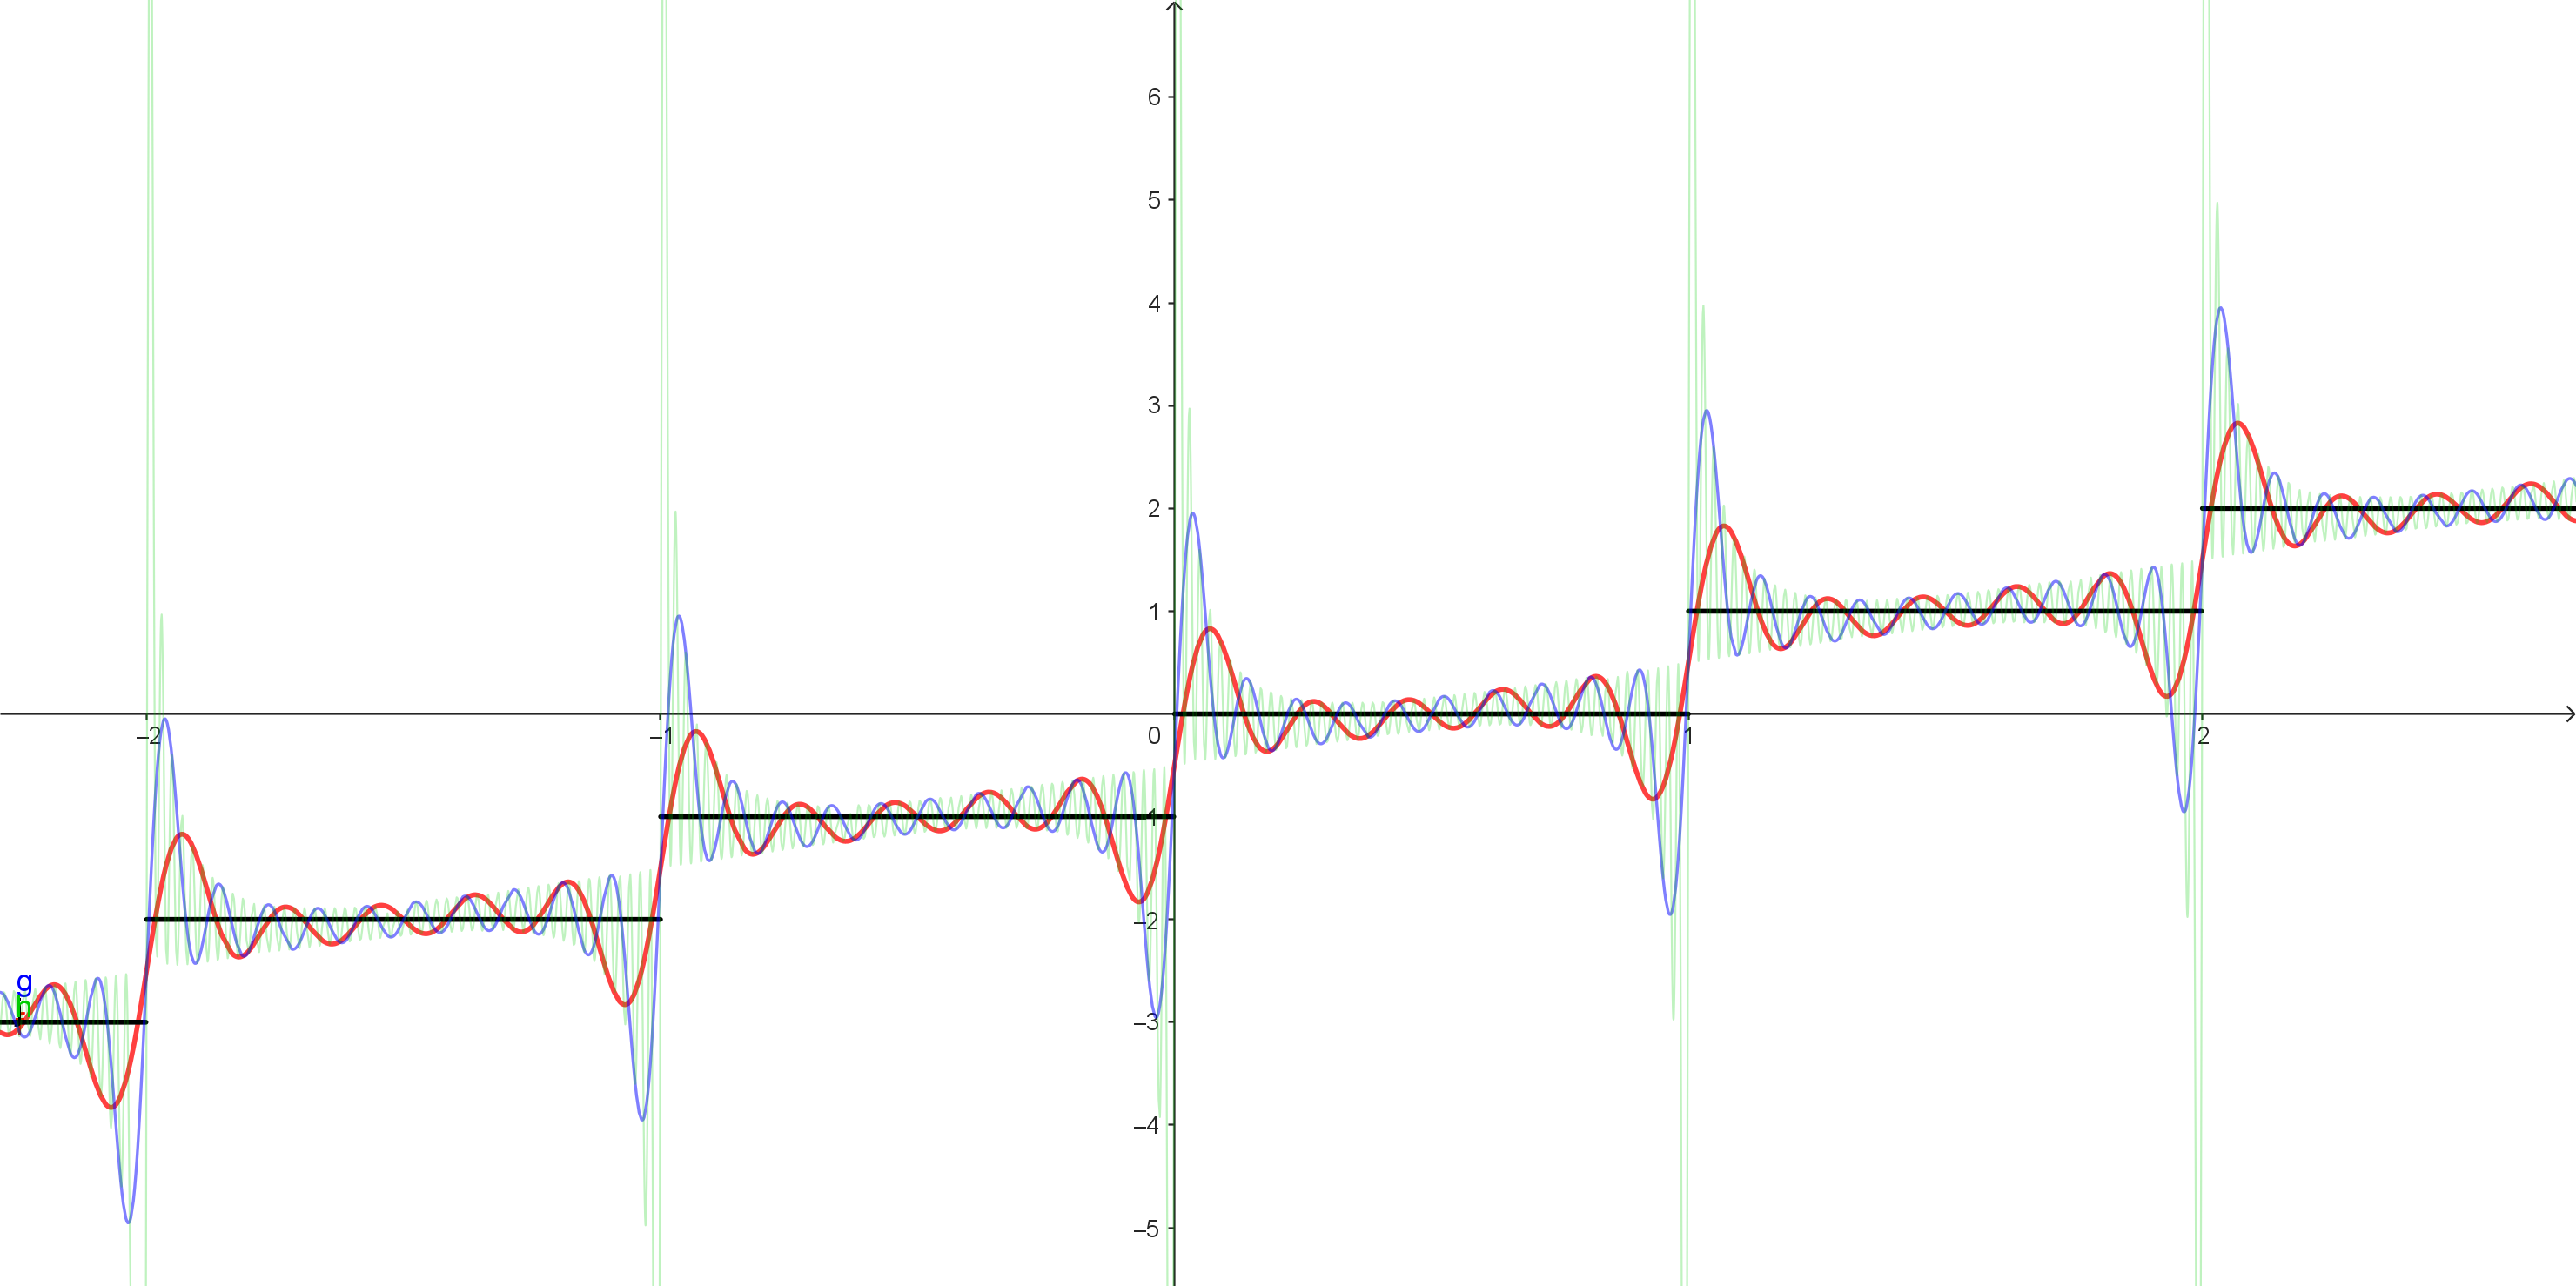
\includegraphics[width=\textwidth]{figure/gibbsphenomenon.png}
  \label{fig:gibbs}
  \caption{Gibbs phenomenon for Equation \ref{eq:floorfourier} with $n=$\textcolor{red}{5},\textcolor{blue}{10},\textcolor{green}{50} and floor(x) in black}
However, due to its discontinuities, Equation \ref{eq:floorfourier} suffers from the Gibbs phenomenon \cite{8e44e918-40ae-3857-bb25-dc12ccf9e7c3}, as illustrated in Figure \ref{fig:gibbs}. 
\begin{figure}[!h]
  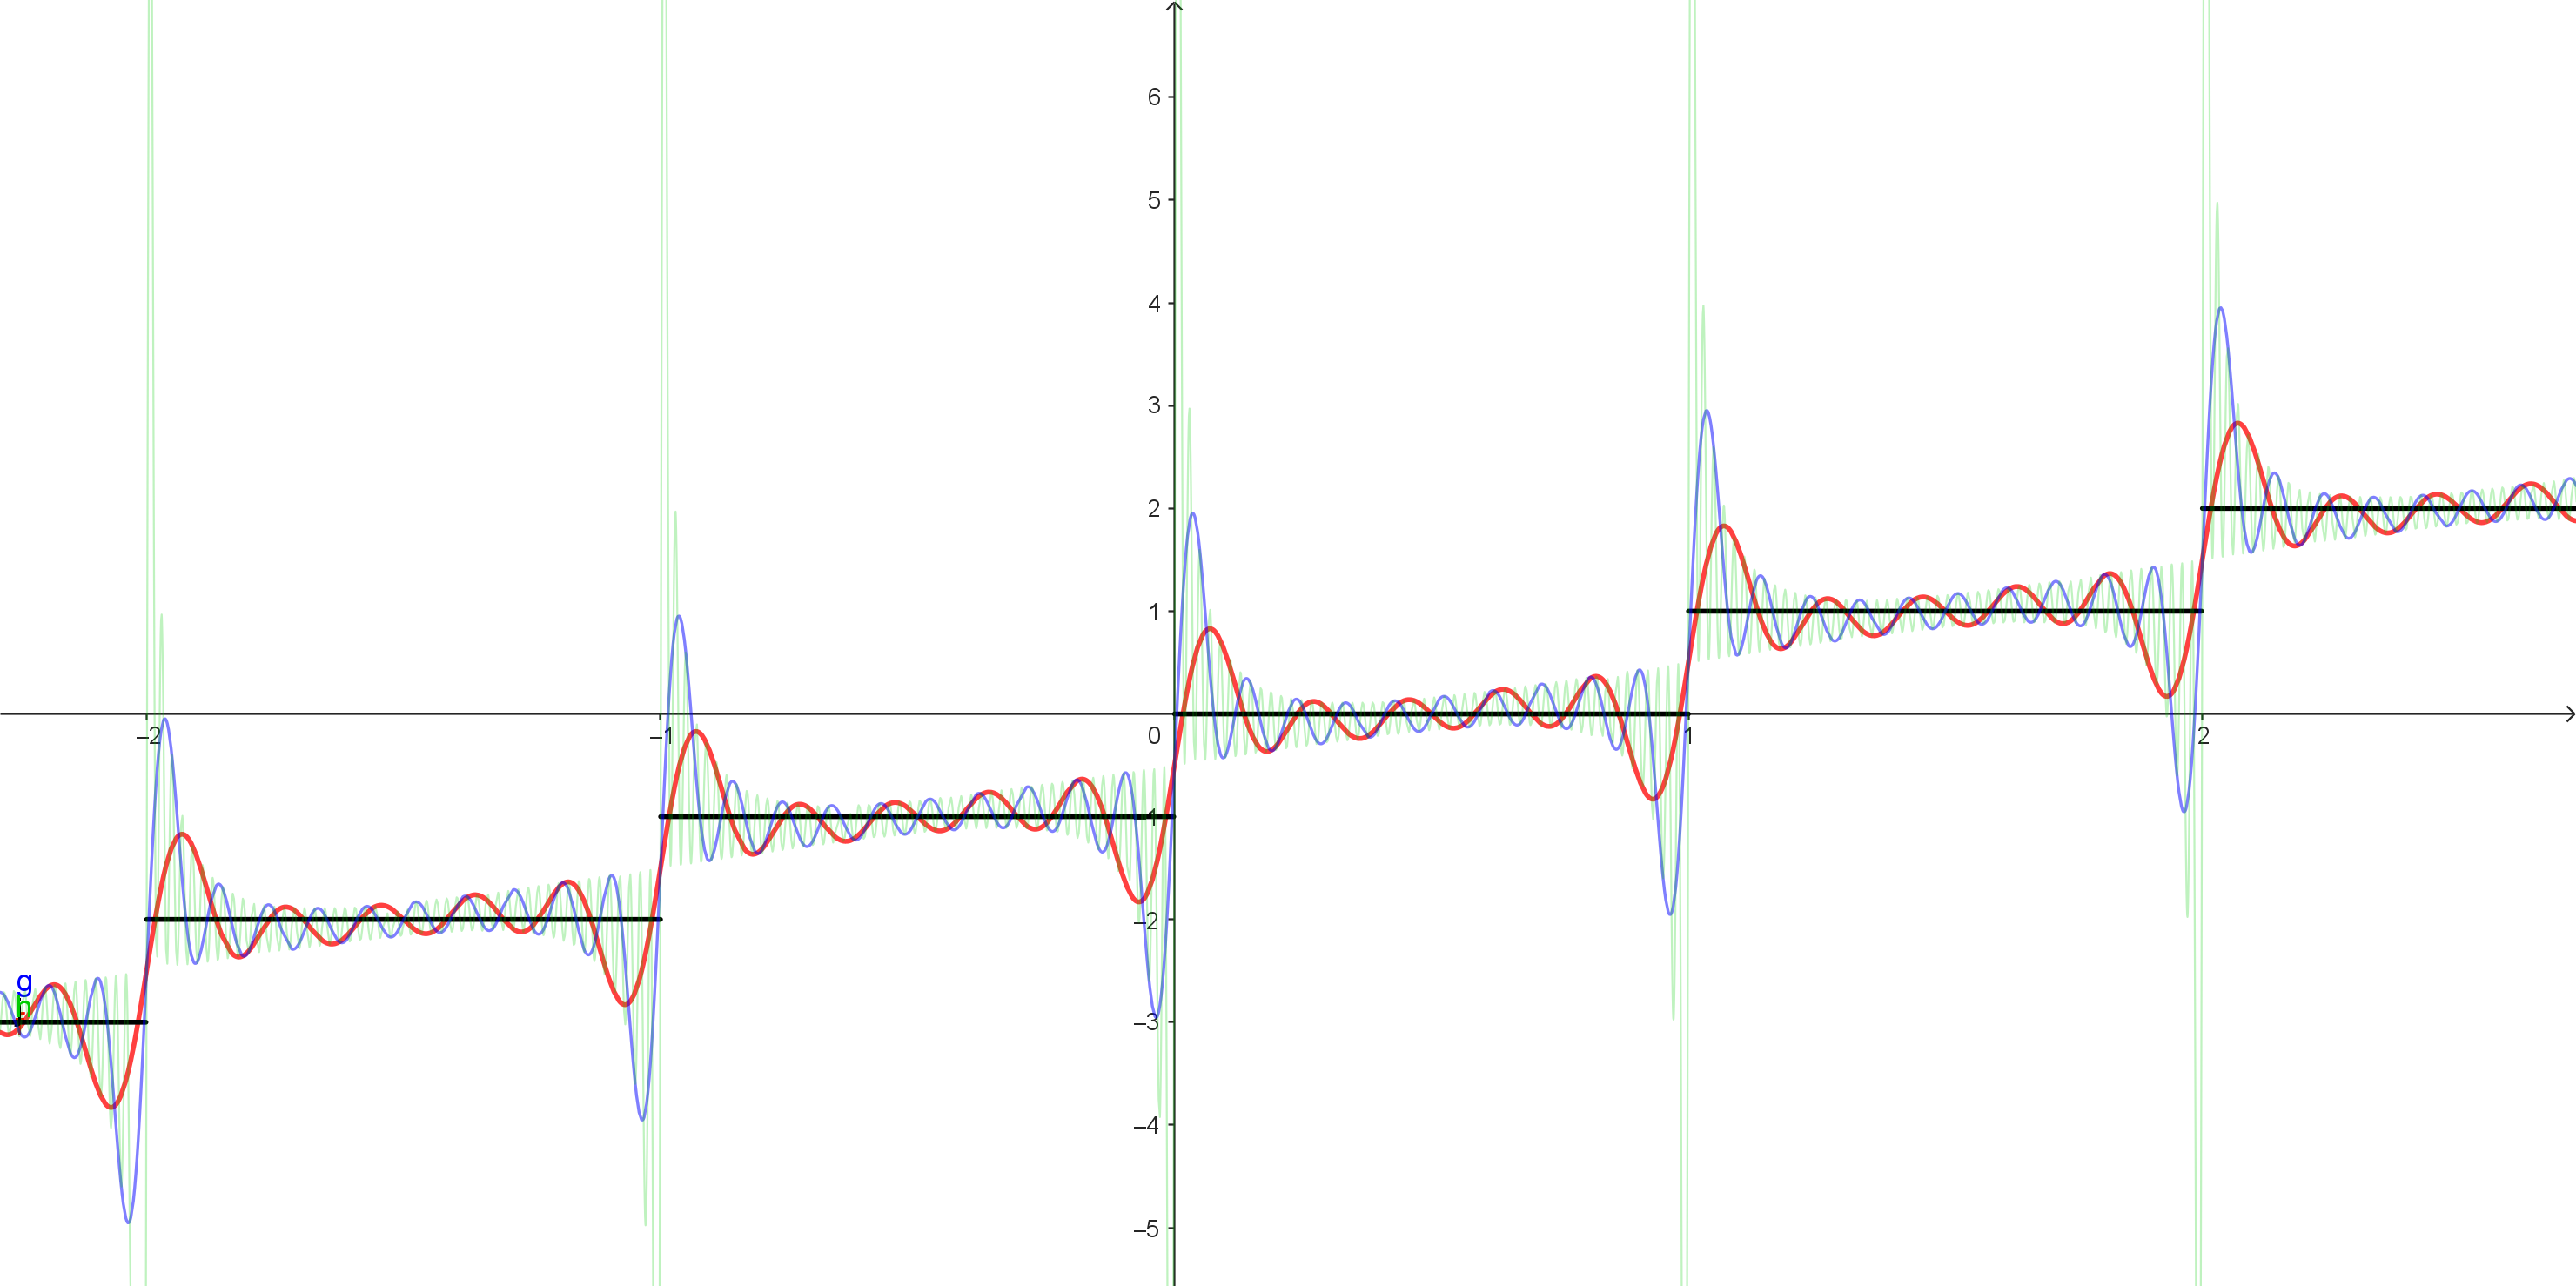
\includegraphics[width=\textwidth]{figure/gibbsphenomenon.png}
  \label{fig:gibbs}
  \caption{Gibbs phenomenon for Equation \ref{eq:floorfourier} with $n=$\textcolor{red}{5},\textcolor{blue}{10},\textcolor{green}{50} and floor(x) in black}
\end{figure}
It means this series cannot be used as it is to mask the floor function in reasonable time. Indeed, we extrapolate through empirical observations that we would require $n=\num{2.5}\times 10^{13}$ to have at least one decimal of absolute precision on the floor computation of $1\times 10^{-16}$. Nonetheless, we will see in this work how we can adapt this Fourier series to compute the floor function in a secure way and in reasonable time with the required precision.
\subsection{Masking}

\section{Masking of the Floor Function}\label{sec:maskfloor}
\subsection{Arithmetization method}
The floor function can be arithmetized using Equation \ref{eq:floorfourier}. However, as stated in Section \ref{subsec:floorfunction}, this method cannot be performed in reasonable time. We thus elaborate a strategy to optimize this arithmetization.

\subsubsection{Absolute Precision} 
The first idea relies on constructing the floor of $x\in\mathbb{R}$ rather than computing it. Indeed, if we can compute the floor of $x$ with one decimal of precision, we can then multiply the result by $10$ and then reapply our computation to the new value $y=10\times \lfloor x\rfloor_1$. Thus, we have the following proposition:
\begin{proposition}\label{prop:floorprec}
  Let $x\in\mathbb{R}$. Let $y = 10\times\lfloor x\rfloor_1$. Then $\lfloor y \rfloor_1 /10 \equiv_2 \lfloor x \rfloor_2$.
\end{proposition}
\begin{proof}
  Let recall that $\lfloor x \rfloor_1 = \lfloor x \rfloor + 0.0 \|[0;9]^*$. Thus, $y=10\times\lfloor x \rfloor_1=\lfloor x\rfloor\|0+0.[0;9]^*$ as multiplying by $10$ can be seen as a left-shift in base $10$. By computing the floor of $y$ with absolute precision $1$ we have $y_1=\lfloor y \rfloor_1 = \lfloor x \rfloor\|0 + 0.0\|[0;9]^*$. Finally, $ y_1/10 = \lfloor x \rfloor + 0.00\|[0;9]^*\equiv_2 \lfloor x \rfloor_2$ as dividing by $10$ can be seen as a right-shift in base $10$.  
\end{proof}
Thus, we can use Proposition \ref{prop:floorprec} to construct the floor of $x$ with the following Algorithm \ref{alg:floorconstruct}:

\begin{algorithm}[H]
  \caption{ConstructFloor($x,prec$)}
  \label{alg:floorconstruct}
  \KwData{$x\in\mathbb{R}$ and the precision $prec\in\mathbb{N}$}
  \KwResult{$\lfloor x\rfloor_{prec}$}
  \For{\texttt{i from 0 to prec-1}}{
    $y \leftarrow \lfloor x \rfloor_1$\;
    $x \leftarrow 10\times y$\;}
    \Return{$x\times 10^{-prec}$}
\end{algorithm}

\begin{theorem}\label{thm:floorprec}
  Let $x\in\mathbb{R}$. Algorithm \ref{alg:floorconstruct} returns $\lfloor x \rfloor_{prec}$ for precision $prec$.
\end{theorem}
\begin{proof}
  We use a recursive proof. The initial state is proven by Proposition \ref{prop:floorprec}. Let Theorem \ref{thm:floorprec} be true for precision $prec-1$. We have $X=\lfloor x \rfloor_{prec-1}$ the output of Algorithm \ref{alg:floorconstruct}. We reapply Algorithm \ref{alg:floorconstruct} to $X\times 10^{prec-1}$ but with precision $1$ and then divide by $10^{prec-1}$. This is stricly equal to applying Algorithm \ref{alg:floorconstruct} with precision $prec$. Algorithm \ref{alg:floorconstruct} with precision $1$ is proven by Proposition \ref{prop:floorprec}. Thus, we have $\lfloor X \rfloor_1 = \lfloor x\rfloor \| \{0\}^{prec-1} + 0.0\|[0;9]^*$. By dividing by $10^{prec-1}$, we shift all the zeros stored in the integer part of $X$ into the fractional part. Thus we have $\lfloor X \rfloor_1 /10^{prec-1} = \lfloor x \rfloor + 0.\{0\}^{prec}\|[0;9]^* \equiv_{prec} \lfloor x \rfloor_{prec}$. We thus proved Theorem \ref{thm:floorprec}.
\end{proof}

%All we need now is a function able of computing $\lfloor x \rfloor_1$ in reasonable time. 
\subsubsection{Relative Precision}
We discuss how to achieve absolute precision from relative precision. In relative precision, we have the possibility that the error from the result can be negative. This results in $\lfloor x \rfloor_n^\alpha = \lfloor x \rfloor - 0.\{0\}^{n}\|[0;9]^*=\lfloor x \rfloor-1 + 0.\{9\}^{n}\|[0;9]^* $. Thus, we cannot construct the floor function using directly $\lfloor x \rfloor_n^\alpha$, as in Algorithm \ref{alg:floorconstruct}. We introduce a second idea: controlled bias.

\medskip

\noindent We have the following Proposition \ref{prop:floorbias}:
\begin{proposition}\label{prop:floorbias}
  Let $x\in\mathbb{R}$. Then $\lfloor x\rfloor_1 \equiv_1 \lfloor x \rfloor_2^\alpha + \alpha\times10^{-2}$.
\end{proposition}
\begin{proof}
  We have two cases to cover: \begin{enumerate}
    \item The error is negative. Thus $-\alpha\times 10^{-2} < \lfloor x \rfloor_2^\alpha - \lfloor x \rfloor \leq 0$ and $0 < \lfloor x \rfloor_2^\alpha + \alpha\times 10^{-2} - \lfloor x \rfloor \leq \alpha\times 10^{-2} < 1\times 10^{-2}$. Thus, in this case, we have $\lfloor x \rfloor_2^\alpha + \alpha\times 10^{-2} \equiv_2 \lfloor x \rfloor_2$ and by construction of $\lfloor x \rfloor_n$, we have $\lfloor x \rfloor_2^\alpha + \alpha\times 10^{-2} \equiv_1 \lfloor x \rfloor_1$.
    \item The error is positive. Thus $0 \leq \lfloor x \rfloor_2^\alpha - \lfloor x \rfloor < \alpha\times10^{-2}$ and $\alpha\times10^{-2} \leq \lfloor x \rfloor_2^\alpha + \alpha\times 10^{-2} - \lfloor x \rfloor \leq 2\alpha\times 10^{-2}$. This implies $0<\lfloor x \rfloor_2^\alpha + \alpha\times 10^{-2} - \lfloor x \rfloor<1\times10^{-1}$. Thus, in this case, we have $\lfloor x \rfloor_2^\alpha + \alpha\times 10^{-2} \equiv_1 \lfloor x \rfloor_1$.
  \end{enumerate}
  We demonstrate that we can have an absolute precision of $1$ from a relative precision of $2$.
\end{proof}

However, we can improve upon Proposition \ref{prop:floorbias} by limiting the maximum value of $\alpha$. We have the following proposition:\begin{proposition}\label{prop:floorbiasopt}
  Let $x\in\mathbb{R}$ and $\alpha<\num{0.5}$. Then $\lfloor x\rfloor_1 \equiv_1 \lfloor x \rfloor_1^\alpha + \alpha\times10^{-1}$.
\end{proposition}
\begin{proof}
  We have already proven in Proposition \ref{prop:floorbias} that for the negative bias, $\lfloor x \rfloor_1^\alpha + \alpha\times 10^{-1} - \lfloor x \rfloor \leq \alpha\times 10^{-1}$. As $\alpha<0.5$, we have $\lfloor x \rfloor_1 \equiv_1 \lfloor x \rfloor_1^\alpha$. For the postive bias, according to Proposition \ref{prop:floorbias} we have $\alpha\times10^{-1} \leq \lfloor x \rfloor_1^\alpha + \alpha\times 10^{-1} - \lfloor x \rfloor \leq 2\alpha\times 10^{-1}$. As $\alpha<\num{0.5}$, $2\alpha\times 10^{-1}<1\times 10^{-1}$. We have $\lfloor x \rfloor_1 \equiv_1 \lfloor x \rfloor_1^\alpha$.
\end{proof}

\subsubsection{Fourier Series}
We now need a way of computing the floor function with a relative precision of at least $2$ in reasonable time. Our final idea revolves around aborting Equation \ref{eq:floorfourier} early for a small value of $n$. Then, we reapply Equation \ref{eq:floorfourier} on the new value, with a small twist:

\begin{algorithm}[H]
  \caption{ArFloorStep($x,n,iter$)}
  \label{alg:floorstep1}
  \KwData{$x\in\mathbb{R}\backsim\mathbb{Z}$, the series limiter $n\in\mathbb{N}$ and the number of iterations $iter\in\mathbb{N}$}
  \KwResult{$\lfloor x \rfloor_2^\alpha+\frac{1}{2}$}
  \For{\texttt{i from 0 to iter-1}}{
    $x \leftarrow x + \frac{1}{\pi}\sum_{k=1}^{n}\frac{sin(2\pi k x)}{k}$\;
  }
  \Return{$x$}
\end{algorithm}
Instead of computing the floor function, Algorithm \ref{alg:floorstep1} gives the floor function with a positive bias of $\frac{1}{2}$. Indeed, applying Equation \ref{eq:floorfourier} and aborting without this bias does not unsure correctness. For instance, for a value close to $0$, using Equation \ref{eq:floorfourier} with a small $n$ results in $-\frac{1}{2} + e$, with $e$ small. Reapplying Equation \ref{eq:floorfourier} will give $-\frac{1}{2}+e-\frac{1}{2}+e_2 \approx -1$ as a result, which is not correct. Thus, it is important to remove $-\frac{1}{2}$ and only apply it after the successive early aborts and reapplications. As an example, Algorithm \ref{alg:floorstep1} is proven by Theorem \ref{thm:floorstep1} for a specific set of parameters:

\begin{theorem}\label{thm:floorstep1}
  Let $x\in(0;1)\subset\mathbb{R}\backsim \mathbb{Z}$ with up to $19$ decimals, \emph{id est} $x= 0.[0;9]^{19}\|{0}^*$. We set $n=3$ and $\alpha=0.4$. Algorithm \ref{alg:floorstep1} returns $\lfloor x \rfloor_1^\alpha+\frac{1}{2}$ in $24$ iterations.
\end{theorem}
\begin{proof}
  We denote $x + \frac{1}{\pi}\sum_{k=1}^{3}\frac{sin(2\pi k x)}{k}$ by $f(x)$. Let set $(U_n)_{n\in\mathbb{N}}$ such as $U_{n+1} = f(U_n)$. First, we will prove the convergence of $(U_n)_{n\in\mathbb{N}}$. Then, we use the Newton method and a visual proof to demonstrate Theorem \ref{thm:floorstep1}.

  \medskip

  \noindent \textbf{PREUVE DE LA CONVERGENCE A FAIRE!!!!!!}

  \begin{figure}[h!]
    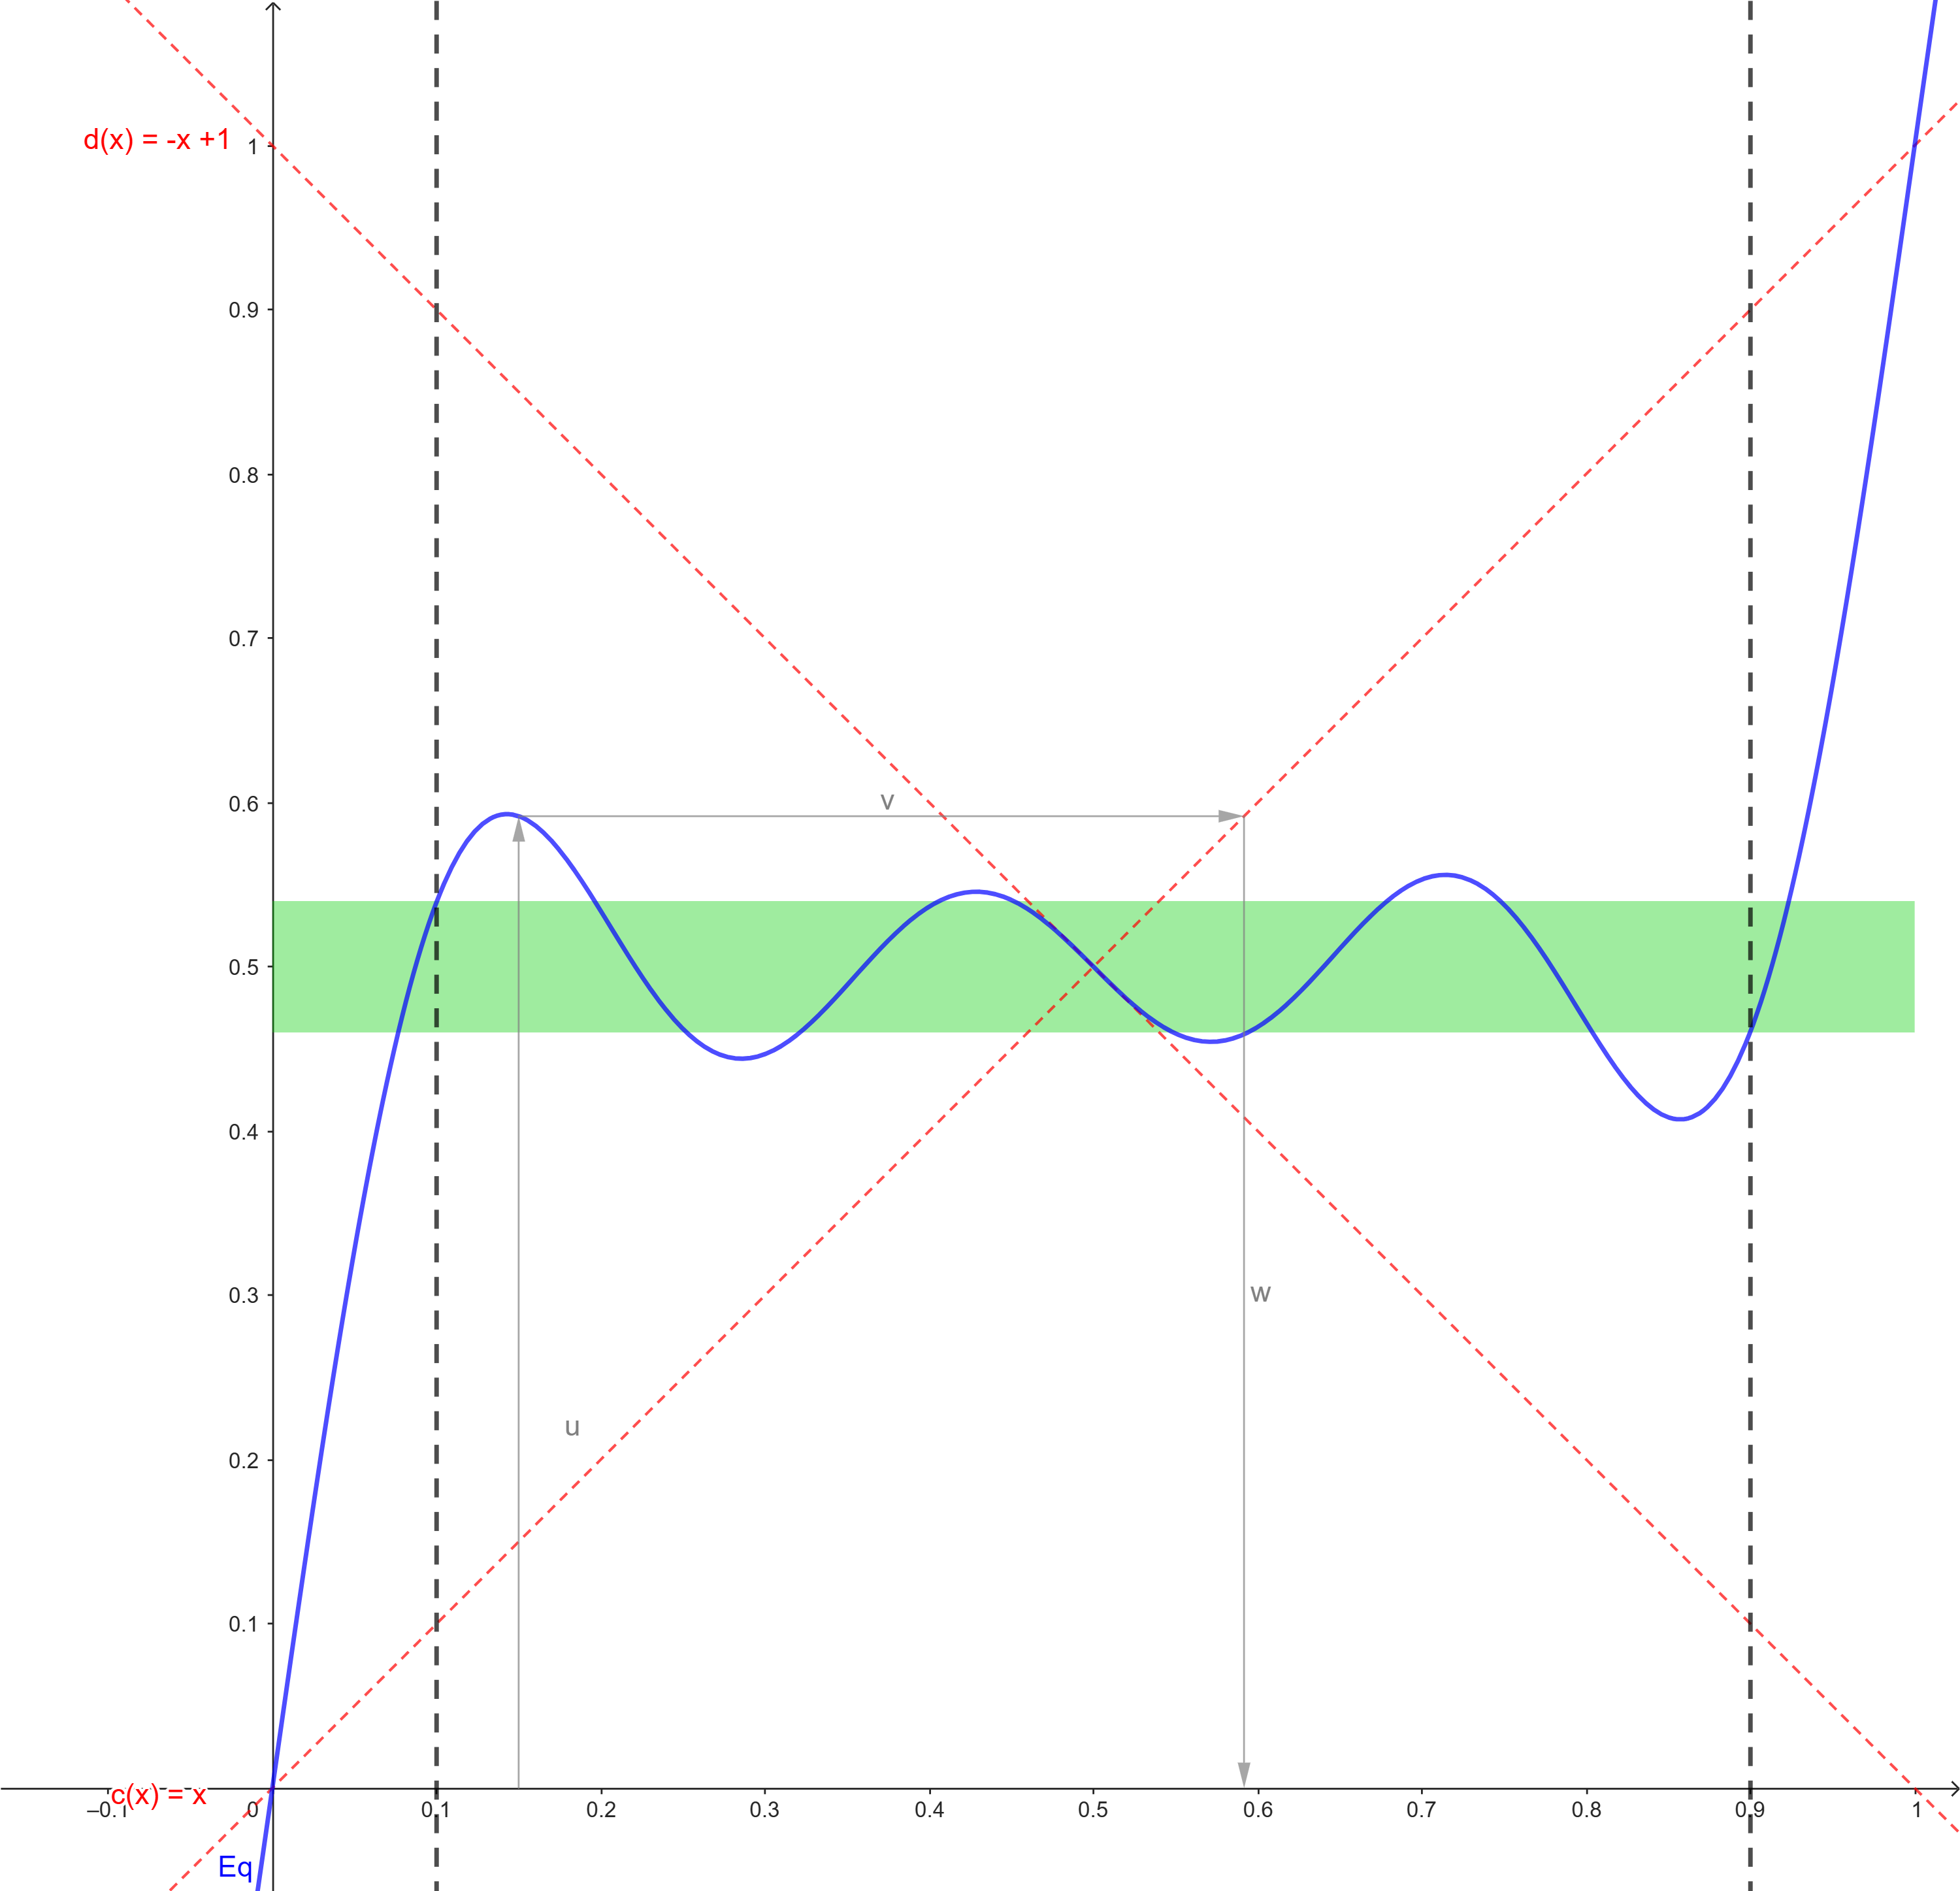
\includegraphics[width =\textwidth]{figure/eqn7Newton.png}
    \caption{Equation \ref{eq:floorfourier} with $n=3$}
    \label{fig:newton3}
  \end{figure}

  For the second part of the proof, we use the Newton method on a graphical representation of $f(x)$(\textcolor{blue}{labeled Eq}). The Newton method, in \textcolor{gray}{grey arrows} in Figure , allows to graphically compute the next term $U_{n+1}$ from $U_n$. We start at the point $(U_n,0)$ ($\num{0.15}$ in this example) and find the point $(U_n,f(U_n))$ (\textcolor{gray}{arrow labeled u}). We then find the point of \textcolor{red}{$c(x)=x$} with ordinate $f(U_n)$ (\textcolor{gray}{arrow labeled v}) and look at its abscissa (\textcolor{gray}{arrow labeled w}), which gives us $U_{n+1}$. Thanks to this method, we can visually compute the number of iterations of Algorithm \ref{alg:floorstep1} required to have $\num{0.46}\leq U_{n+1}\leq \num{0.54}$(\textcolor{green}{green area}). The amount of iterations is shown in Table \ref{tab:n3} (due to the symetric nature of $sin(x)$, we restrict the study on $(0;\num{0.5}]$).

  \begin{table}[!h]
    \caption{Subsets of $(0;\num{0.5}]$ and number of iterations to reach $[\num{0.46};\num{0.54}]$}
    \label{tab:n3}
    \begin{tabularx}{\textwidth}{lcX}
      \toprule
      Number of iterations & &Subsets \\
      \midrule
      1 & &$U_1=[\num{0.0767};\num{0.1002}]\vee[\num{0.1962};\num{0.2522}]\vee[\num{0.3213};\num{0.4060}]\vee [\num{0.4514};\num{0.5}]$\\
      At most 2 & & $U_2=U_1\vee[\num{0.0110};\num{0.0143}]\vee[\num{0.0287};\num{0.0373}]\vee[\num{0.0488};\num{0.0648}]\vee[\num{0.0746};\num{0.263}]\vee[\num{0.3095};\num{0.5}]$\\
      At most 3 & & $U_3=U_2\vee[\num{0.0016};\num{0.002}]\vee[\num{0.0041};\num{0.0052}]\vee[\num{0.007};\num{0.0092}]\vee[\num{0.0107};\num{0.0391}]\vee[\num{0.0469};\num{0.5}]$\\
      \bottomrule
    \end{tabularx}
  \end{table}
\end{proof}

\begin{remark}\label{rem:alpha04}
  The choice of setting $\alpha=\num{0.4}$ in Theorem \ref{thm:floorstep1} is not the most optimal as taking $\alpha=\num{0.5}$ is more advantageous as shown in Proposition \ref{prop:floorbiasopt}. However, by taking $\alpha = \num{0.4}$, we have that Algorithm \ref{alg:floorstep1} returns $\lfloor x \rfloor + err$ such as $\num{0.46}\leq err \leq \num{0.54}$. Thus, by retrieving to this result $0.45$, we have $\num{0.01} \leq err - \num{0.45} \leq \num{0.09}$. By multiplying by $10$, we have $\num{0.1} \leq 10*(err-\num{0.45}) \leq \num{0.9}$. As a result, when applying Algorithm \ref{alg:floorconstruct} we avoid some extreme points and reduce the number of iterations required by Algorithm \ref{alg:floorstep1}. This strategy is not specific to the current set of parameters and will always benefit our method. 
\end{remark}

According to Table \ref{tab:n3}, all values of $x\in[\num{0.1};\num{0.9}]$ converge towards $[\num{0.46};\num{0.54}]$ in less than $3$ iterations. Thus, in accordance with Remark \ref{rem:alpha04} we can limit the number of iterations in the following steps of our floor compuation to only $3$. We can use Algorithm \ref{alg:arfloor} to compute the floor function of $x\in\mathbb{R}\backsim\mathbb{Z}$ in reasonable times.

\begin{algorithm}[H]
  \caption{ArFloor($x,prec$)}
  \label{alg:arfloor}
  \KwData{$x\in\mathbb{R}\backsim\mathbb{Z}$ and the precision $prec\in\mathbb{N}$}
  \KwResult{$\lfloor x \rfloor_prec$}
  $x\leftarrow \emph{ArFloorStep}(x,3,24) -\num{0.45}$\;
  $x \leftarrow 10 \times x$\;
  \For{\texttt{i from 1 to prec-1}}{
    $x \leftarrow \emph{ArFloorStep}(x,3,3) - \num{0.45}$\;
    $x \leftarrow 10 \times x$\;
  }
  \Return{$x \times 10^{-prec}$}
\end{algorithm}

\section{Truncation method : Masked Floor Function}
In this part we will consider $f$ as one of these three funtions : floor, truncature and round. There's some little differences between those functions and we will explain it in times.

\subsection{Overview}
  %\paragraph[short]{Binary64 -- IEEE 754.} 
  Recall that we're working with floating point in a specific representation, the standardized\footnote{Binary64 -- IEEE 754} one,
    it's really important to understand the encoding method because all operation algorithms using floating point are based on. We can define this encoding as follow : 
    let $x \in \mathbb{R}$, $x$ is represented by a tupple of three elements $(s,e,m)$, where $s$, $e$ and $m$ are respectively 1-bit length, 11-bit length and 52-bit length, such as $$x= (-1)^s \times 2^{e-1023} \times (1+m\times 2^{-52})$$
    We call $s$ the sign bit, $e$ the exponent and $m$ the mantissa.% which we must not forget to add an implicit bit. 
    The most important element we will use to construct $f$ between those three is the exponent $e$. Just by analyzing it, we can distinguish three different cases :
    \begin{enumerate}
        \item If $e-1023<0$, the result will be $0$. However, it exists a subtlety if $f$ = round. In this case we must take care of the rounding and test if $e-1022<0$. It's only by not rejecting the case of $e=1022$ that we can compute the correct rounding;
        \item If $e-1075\geq0$, the input $x$ is already an integer, so the output $y$ will be equal to $x$;
        \item If $0\leq e-1023 \leq 51$,the result must be computed by removing the $52-(e-1023)$ decimals, and adjusting the result if $f$ = round. 
    \end{enumerate}
    These three distinguished cases provide a fixed structure shown in \autoref{algo:SecFprBaseInt} for $f$. The main difficulty here is to compute securly all the checks on masked values, and to change in consequence our mantissa, exponent and eventually our sign bit. 

    \subsection{Masked Floor Function}
    The function SecFprBaseInt is the main function to compute masked floor, masked truncature or masked round. Its result depends on the inputed function : gadgets and Zero$_f$ are different. 
    \begin{figure}[h!]
        \centering
        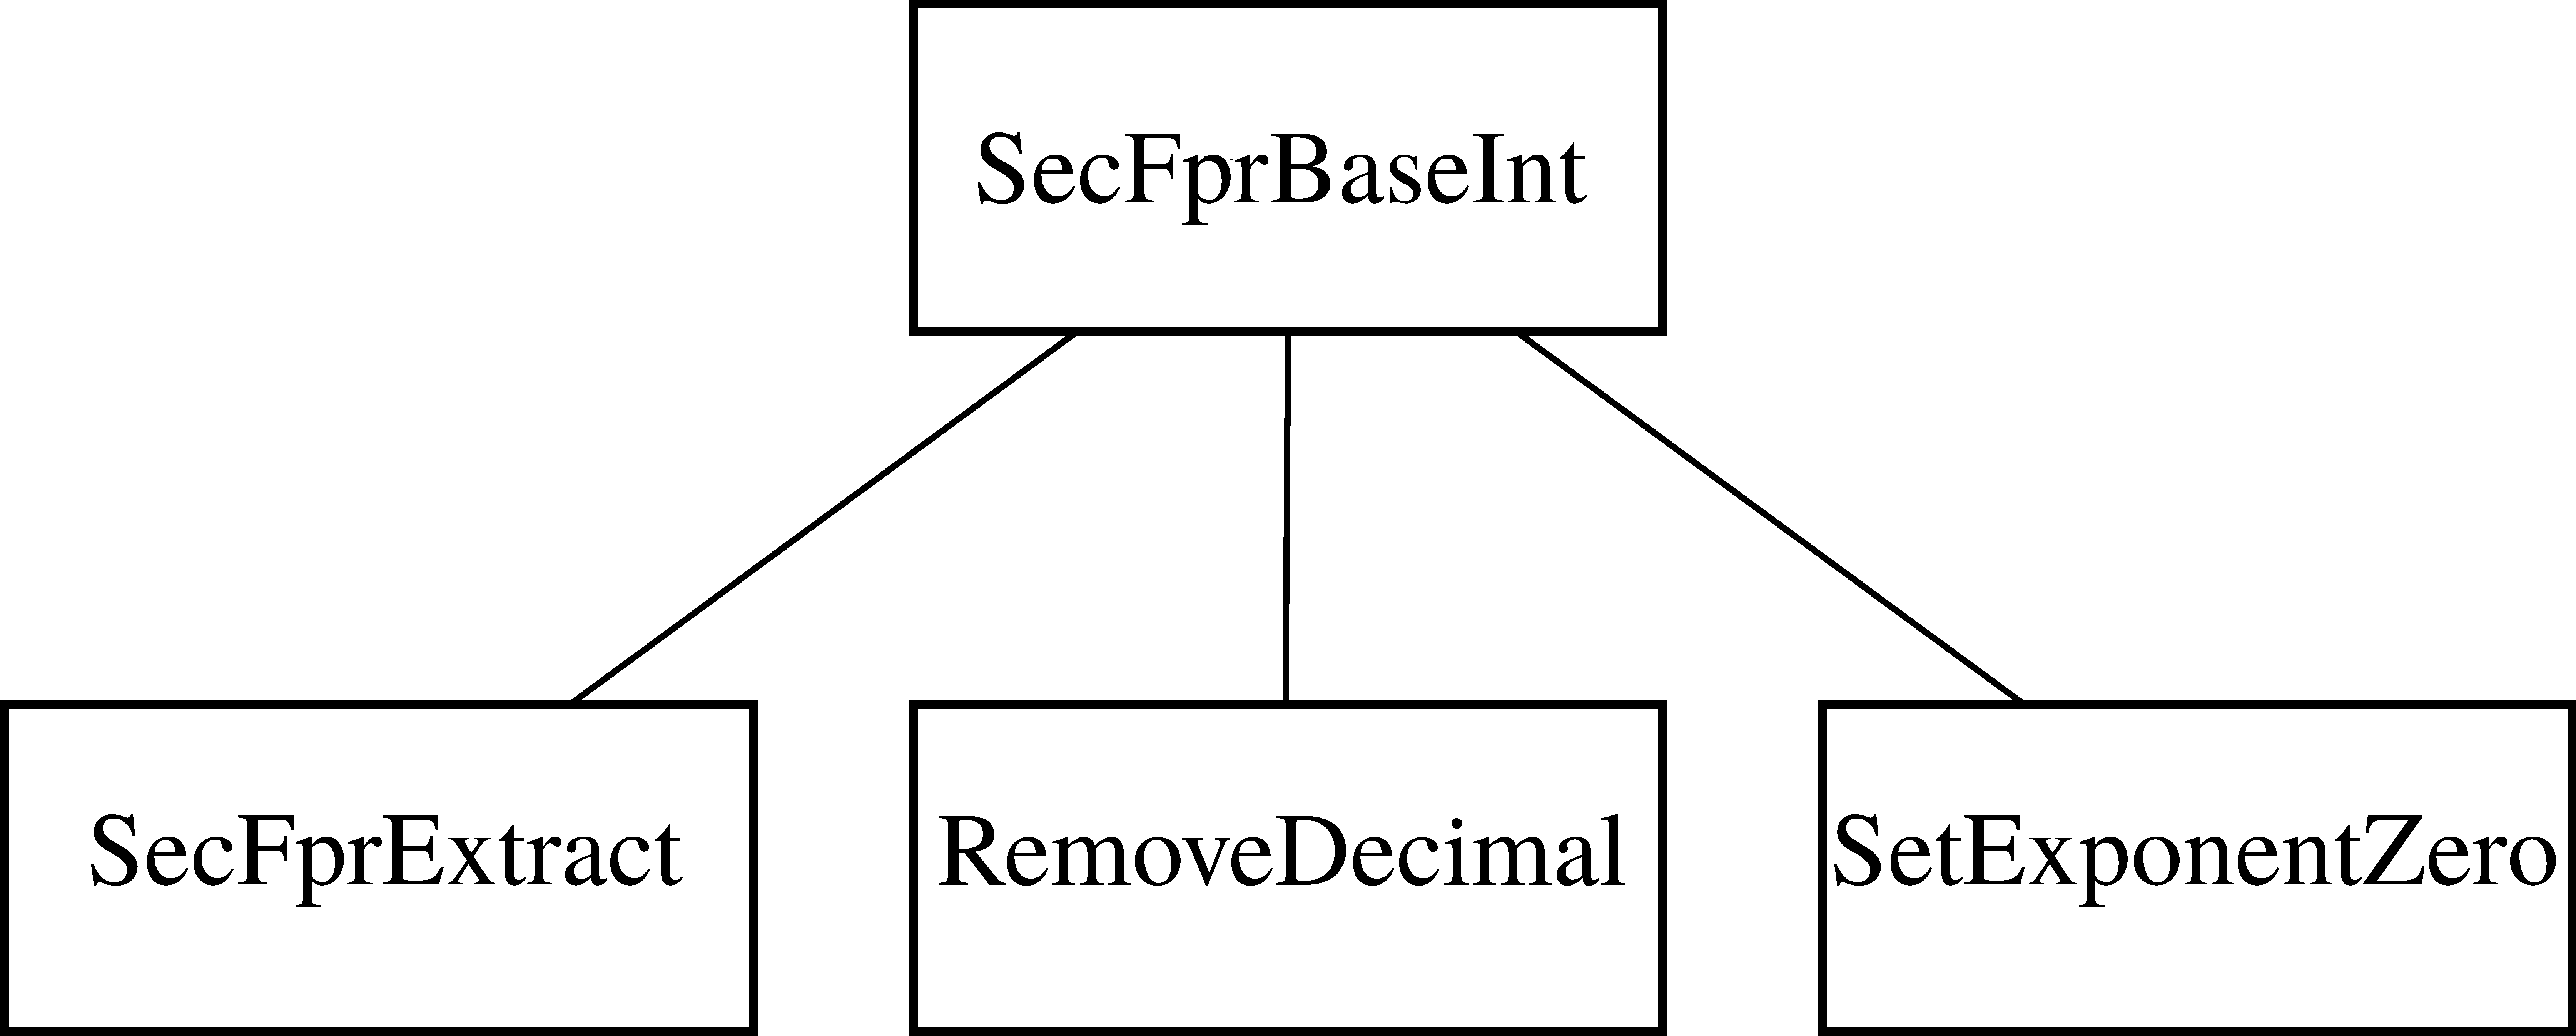
\includegraphics[width=0.5\textwidth]{figure/secpfrhierarchie.pdf}
        \label{fig:hierar}
        \caption{SecFprBaseInt and its gadgets}
    \end{figure}

    In this subsection, suppose $f$ = floor. We will first present the main structure and then present the gadgets. Gadgets from trunc and round function can be found in annexe (the little differences between gadgets will be explain too):
    \begin{itemize}%[label = $\bullet$]
        \item SetFprExtract;
        \item RemoveDecimal$_\text{trunc}$ and SetExponentZero$_\text{trunc}$;
        \item RemoveDecimal$_\text{round}$ and SetExponentZero$_\text{round}$.
    \end{itemize}
    The particularity of our shift method for calculating floor function is that it requires the gadgets proposed by Chen and Chen \cite{Chen_Chen_2024}. So by proposing this method, we are extending their work to mask the Gaussian sampler by using only the gadgets of their creation.
    By way of summary, we propose a table showing the functions used to create our gadgets and the sources from which they come.

    \begin{figure}[h!]
        \begin{center}
            \begin{tabular}{C{2.5 cm} || C{6 cm} C{1.2cm} C{2cm}}
                \hline \textbf{Algorithm} & \textbf{Decription} & \textbf{Security} & \textbf{Reference}\\
                \hline SecAnd   & AND of Boolean shares             & $t$-SNI &  \cite{ishai2003private}, \cite{barthe2016strong}\\
                 SecAdd         & Addition of Boolean shares        & $t$-SNI&  \cite{coron2015conversion}, \cite{barthe2018masking}\\
                 A2B            & Arithmetic to Boolean conversion  & $t$-SNI& \cite{schneider2019efficiently}\\
                 B2A            & Boolean to Arithmetic conversion  & $t$-SNI&  \cite{bettale2018improved}\\
                 RefreshMasks   & $t$-NI refresh of masks           & $t$-NI&  \cite{barthe2016strong}, \cite{bettale2018improved}\\
                 Refresh        & $t$-SNI refresh of masks          & $t$-SNI& \cite{barthe2016strong}\\
                 SecOr          & OR of Boolean shares              & $t$-SNI&  \cite{Chen_Chen_2024}\\
                 SecNonZero     & NonZero check of shares           & $t$-SNI&  \cite{Chen_Chen_2024}\\
                 SecFprUrsh     & Right-shift keeping sticky bit updated  & $t$-SNI&  \cite{Chen_Chen_2024}\\
                 SecFprNorm64   & Normalization to $[2^{63},2^{64})$ & $t$-NI& \cite{Chen_Chen_2024}\\
                \hline
            \end{tabular}
        \end{center}
    \end{figure}

    \begin{algorithm}
        \caption{SecFprBaseInt(x, f)}
        \label{algo:SecFprBaseInt}
        \KwData{64-bit boolean shares $(x_i)_{1\leq i \leq n}$ for value x \\
        A function f : floor, round or trunc.}
        \KwResult{64-bit boolean shares $(y_i)_{1\leq i \leq n}$ for mantissa value y = floor(x)/round(x)/trunc(x).} 
        $((my_i), (ey_i), (sy_i)) \leftarrow$ SecFprExtract($(x_i)$)\;%\tcp*{extract mantissa, exponent and sign}
        $(cx_i) \leftarrow (ey_i)$\;
        $cx_1 \leftarrow ey_1 - \text{Zero}_f$\;%\tcp*{$\text{Zero}_f$ = 1023 for floor }%and trunc, $\text{Zero}_f$ = 1022 for round}
        $(c_i) \leftarrow$ A2B($(cx_i^{(16)})$)\; 
        $(c_i) \leftarrow$ SecNonZero($(c_i)$)\tcp*{check if the exponent is negative}
        $(b_i) \leftarrow (\neg(-c_i))$\;
        Refresh($(cx_i)$)\;
        $(my_i) \leftarrow$ SecAnd($(my_i), (b_i)$)\;%\tcp*{if c = 0,  my = mx and if c = 1, my = 0 }
        $(my_i), (ey_i), (Rnd_i) \leftarrow$ RemoveDecimal$_f((my_i), (ey_i), (sy_i), (cx_i)$)\;% \tcp*{depends on f}
        $(my_i), (ey_i) \leftarrow$ SecFprNorm64($(my_i),(ey_i)$)\;
        $(my_i) \leftarrow (my_i >> 11)$\;
        $(my_i) \leftarrow$ $(my_i^{[52:1]}) $\;
        $ey_1 \leftarrow ey_1 + 11$\;
        $(ey_i), (sy_i) \leftarrow$ SetExponentZero$_f((ey_i), (b_i), (s_i), (Rnd_i))$\;%\tcp*{set ey at 0 if f(x)=0}
        $(y_i^{(64)}) \leftarrow (sy_i) $\;
        $(y_i^{[63:53]}) \leftarrow (ey_i) $\;
        $(y_i^{[53:1]}) \leftarrow (my_i) $\;
      \Return{$(y_i)$}\;
      \end{algorithm}
      \subsubsection{SetFprBaseInt$_\text{floor}$ -- \autoref{algo:SecFprBaseInt}}
      As explained in overview, these three functions can be summarised in a global structure. 
      What will differentiate the three functions will in fact be the gadgets and the Zero$_f$ parameter.
      To perform the floor function, we first extract the data from the encoding and place it in three variables $s_y, e_y$ and $m_y$, which will be linked directly to the output of the algorithm. 
      By extracting this data footnote{Pseudo-code in appendix: SecFprExtract -- \autoref{algo:SecFprExtract }}, we carry out a few operations on the mantissa and the exponent to match the conventions of Chen's implementation..
        Indeed, the input $x$ is a 64-bit boolean share, consequently we'll have to transform the exponent into a 16-bit arithmetic share by performing a boolean to arithmetic conversion.
        Another important thing to add is the bit implicit in the mantissa. 
        This bit which is not present in the $x$ information, in order to save one bit and gain in precision, is nevertheless very important.
        In particular, it enables us to normalise our shares correctly.
        Once these changes have been made, we can start working on the exponent.

        Without any surprise, the first step consists of checking whether the result is an obvious zero or not.
        To do so, we compare $e_y$ and Zero$_f$ -- which is the correponding exponent to  $1=2^0$ -- by calcultating $c_x = e_y - \text{Zero}_f$.
        If $cx$ is negative, $\mid x \mid <1$ and all decimals can be removed by putting $my = 0$.
        We just need to be carefull at the end of the algorithm because of some particular cases\footnote{For example, if $-1<x<0$, we need to return encoding -1, not zero.}.
        This step without taking care of particular case corresponds in reality to the truncature.
        Otherwise, the $m_y$ mantissa will remain unchanged to be adjusted during the next steps.

        A mathematical explanation of Zero$_f$'s choice can be summurize in a few simple calculus.
        In case $f$ = floor or trunc, Zero$_f = 1023$.
        Indeed if $e_y -1023 <0$, $$2^{e_x-1023} \times (1+m_x\times 2^{-52})\quad\leq \quad 2^{-1} \times (1+m_x\times 2^{-52}) \quad< \quad 1$$ 
        We remark a difference for $f$ = round.
        The main reason of this difference is that we want to avoid to reject the case where the binary decomposition of $x$ contains a $1$ at indices $2^{-1} = 0.5$, 
        since we will no longer be able to round off the final result.
        This justify the choice of  Zero$_f =1022$ for rounding function.
        This time, if $e_y -1022 <0$: 
        $$2^{e_x-1023} \times (1+m_x\times 2^{-52})\quad\leq \quad 2^{-2} \times (1+m_x\times 2^{-52}) \quad< \quad 0.5$$ 
        
        To sum up, after the first step, only $my$ can change. The two values it can take are $my$ it-self (no changes) or $0$.
        The second step 
        The second step removes the decimals by shifting them to the right, using RemoveDecimal -- \autoref{algo:RemoveDecimal_floor}. 
        As this algorithm does not normalise the mantissa, we then apply the SecFprNorm64 function, !!!!!!!! followed by a refresh (SecFprNorm64 is a $t$-NI gadgets) and !!!!!!!!!!! a computation of shifted $my$ and $ey$ to set the mantissa back to bits $[52:1]$ and update $ey$.
        Finally, the last step in the algorithm, before reformatting the initial encoding, is to apply the specific encoding of "0" if this is the result to be returned.
        To do this, we apply the SetExponentZero$_f$ function -- \autoref{algo:SetExponentZero_floor}. 
        \begin{algorithm}
            \caption{RemoveDecimal$_{\text{floor}}((my_i), (ey_i), (sy_i), (cx_i))$}
            \label{algo:RemoveDecimal_floor}
            \KwData{64-bit boolean shares $(my_i)_{1\leq i \leq n}$ for mantissa value my; \\
            16-bit arithmetic shares $(ey_i)_{1\leq i \leq n}$ for exponent value ey; \\
            1-bit boolean shares $(sy_i)_{1\leq i \leq n}$ for sign value sy\\
            16-bit arithmetic shares $(cx_i)_{1\leq i \leq n}$ for value cx = ex-2013.}
            \KwResult{64-bit boolean shares $(my_i)_{1\leq i \leq n}$ for mantissa value $my >> (52 - cx)$; \\
                      16-bit arithmetic shares $(ey_i)_{1\leq i \leq n}$ for exponent value $ey +(52 - cx)$;} 
            $cx_1 \leftarrow cx_1 - 52$\;%\tcp*{check if 0$\leq$c$<$51}
            $(c_i) \leftarrow$ A2B($(cx_i)$)\;
            $(cp_i) \leftarrow (c_i^{(16)})$\;
            $(cp_i) \leftarrow$ SecNonZero($cp_i$)\;
            $(c'_i) \leftarrow (- cp_i)$\;%\tcp*{if cp = 0 cx = 0. if not cx = cx }
            $(c_i) \leftarrow$ SecAnd($(c_i), (c'_i)$)\;
            $(cx_i) \leftarrow$ B2A($(c_i)$)\;
            $(cd_i) \leftarrow (-cx_i)$\;
            $(my_i), (rot_i) \leftarrow$ SecFprUrsh$_f$($(my_i), (cd_i)$)\;%\tcp*{$my >> 52 - cx$ and $rot = my^{[52-cx:1]}$}
            $(b_i) \leftarrow$ SecNonZero($(rot_i)$)\;%\tcp*{if $b=0$, $x \in \mathbb{N}$, else $x\in \mathbb{R}/\mathbb{N}$ }
            $(cp_i) \leftarrow$ SecAnd($(cp_i), (sy_i)$)\; 
            $(cp_i) \leftarrow$ SecAnd($(cp_i), (b_i)$)\; 
            $(my_i)\leftarrow$ SecAdd($(my_i), (cp_i)$)\;%\tcp*{add 1 only if $s = 1$ and if $x \in \mathbb{R}/\mathbb{N}$}
            $(ey_i) \leftarrow (ey_i + cd_i)$\; 
          \Return{(Refresh$(my_i)$, Refresh$(ey_i))$}\;
          \end{algorithm}
    \subsubsection{RemoveDecimal$_\text{floor}$ -- \autoref{algo:RemoveDecimal_floor}}
    As we explained at the beginning of this section, we need to remove the decimals from the input number.
    After checking a first result, the mantissa is equal to 0, if $e-\text{Zero}_f<0$, or has remained unchanged.
    This leaves us with the case where a shift is needed. To do so, we write $cx = e - 1023$ as the shift to be performed.
    The case where $cx<0$ has already been treaten by modifying (or not) the mantissa, whatever shift is made, we would have $0>>cx = 0$.
    If $cx=\geq52$, $x$ is already in the correct form. In fact, we have : 
    $$\mid (-1)^s \times 2^{cx} \times(1+m\times 2^{-52})\mid \quad \geq \quad 2^{52} \times(1+m\times 2^{-52})\quad = \quad2^{52} + m \in \mathbb{N}$$
    To avoid removing information if it isn't needed, we replace $cx$ by $0$.
    Be careful if we want to round a number : it's important to compare $cx$ to $53$ instead of $52$. The reason is that we first subtract to $ey$ $1022$ instead of $1023$ when we were checking is the result was 0 or not. So here we need to add 1.
    If $0\leq e_y - 1023 \leq 51$, we need to modify the mantissa to remove -- if necessary-- the decimals.
    Remarks that even in this case, the mantissa can be in the good format. For example if $x = 5$, we have $0\leq e_y-1023 = 1025-1023 = 2 \leq 51$ and $x$ is an integer.
    
    After verifying is $x$ is or isn't a "big" number, i.e. without decimal in its representation, we can shift\footnote{
    In pseudo-code the subtraction is implicite due to the format of a masked value.} $my$ by $cd=52-cx$ by applying a modified \footnote{If
    we want to use Chen's algorithm, it's possible. We just need to compute one shift less then described in our algorithm and then compute an extra shift manually. The disadvantges of using it, is that you need to check if $cx$ is different from $0$ 
    -- to not compute a shift if it isn't needed -- and the cost of computing the sticky bit.} SecFprUrsh$_f$ -- \autoref{algo:SecFprUrsh}: 
    we don't want to keep the sticky bit, so we just removed this part.
    We had an extra output, returning the part we removed.
    Shift a value is a good thing, but that's not exactly the floor function. After this step we just have the truncature.
    When $x$ positive there's no problem at all, floor function is equal to truncature. But when $x$ is negative there is one. It cames from floor properties. Indeed if $x<0$ : 
    \begin{equation}
        \label{eq:floorneg}
        \text{floor}(-x)  = \Bigg\{ \begin{array}{cc}
            \text{trunc}(-x) &  \text{if } x\in\mathbb{N}\\
            \text{trunc}(-x) -1 &  \text{if } x\in\mathbb{R}/\mathbb{N}
         \end{array}
    \end{equation}

    On one hand, checking if $x$ is negative is quite easy : we just have to take a look at if $sy$ is equal to 1.
    On the other hand, checking that $x$ is an integer is trickier. This is where the second modification to SecFprUrsh$_f$ comes in handy. As this function performs a rotation, the bit information is retained until a mask is applied to calculate the shift. 
    We therefore decided to invert the mask in order to retain the suppressed information. If this information has zero Hamming weight
    then $x$ is an integer. We can then use the SecNonZero gadget on this information, which will return $0$ if $x$ is an integer, and 1 if not.
    We denote this result $b=$ SecNonZero(($my_i^{[52 - c_x:1]}$)). 
    In the following truth table (\autoref{figure:flooradjust}) if the result $cp = $ $s$ AND $b$ is $1$, the mantissa must be changed.
    \begin{figure}
        \begin{center}
            \begin{tabular}{C{0.5cm} C{0.5cm} || C{3 cm} L{3cm}}
                \hline $sy$ & $b$ &$cp$ = $sy$ AND $b$ & Interpretation\\
                \hline 
                0 & $b$ & 0 & Positive number\\
                1 & 0  & 0 & $x$ is an integer\\
                1 & 1  & 1 & Negative real\\ \hline
            \end{tabular}
        \end{center}
        \caption{Do we need to subtract $s$: Truth table}
        \label{figure:flooradjust}
    \end{figure}
    Another question is now : how to subtract $s$ from the mantissa if the mantissa is always positive? 
    The sign of $x$ is only define by $sy$, so $\mid x\mid = 2^{ey-1023}\times(1 + my\times 2^{-52})$.
    We already know that if $x$ is positive or an integer,$my = my \pm 0 = my \pm cp$.
    Now let's focus on $x$ a non integer negative number. Let $x$ be a positive real, from \autoref{eq:floorneg}, we can write :
    \begin{equation}\label{eq:floorabs}
        my =\: \mid \text{floor}(-x)\mid \:=\: \mid \text{trunc}(-x) - 1\mid
    \end{equation}
    By using $\mid \text{trunc}(-x) \mid \:=\: \mid -\text{trunc}(x)\mid \:$, we can transform \autoref{eq:floorabs} :
    \begin{equation}\label{eq:floorabs2}
        my =\: \mid \text{floor}(-x)\mid \:=\: \mid -\text{trunc}(x) - 1\mid \:=\: \mid \text{trunc}(x) + 1\mid \:= my + cp
    \end{equation}
    \begin{algorithm}
      \caption{SecFprUrsh$_{\text{floor}}((my_i), (cx_i))$}
      \label{algo:SecFprUrsh}
      \KwData{ 6-bit arithmetic shares $(cx_i)_{1\leq i \leq n}$ for value cx; \\
      64-bit boolean shares $(my_i)_{1\leq i \leq n}$ for sign value $my$.}
      \KwResult{64-bit boolean shares $(my'_i)_{1\leq i \leq n}$ for value $my>>cx$\\
      64-bit boolean shares $(rot_i)_{1\leq i \leq n}$ for value $my^{[cx : 1]}$.} 
        $(m_i)_{1\leq i \leq n} \leftarrow ((1<<63), 0, \cdots, 0)$\;
        \For{\texttt{i from 1 to n}}{
          Right-Rotate $(my_i)$ by $cx_j$\;
          $(my_i) \leftarrow$ RefreshMasks($(my_i)$)\;
          Right-Rotate $(m_i)$ by $cx_j$\;
          $(m_i) \leftarrow$ RefreshMasks($(m_i)$)\;
        }
        $len \leftarrow 1$\;
        \While{$len\leq 32$}{
          $(m_i) \leftarrow (m_i \oplus (m_i>>len))$\;
          $len \leftarrow len<<1$\;
        }
        $(my'_i) \leftarrow$ SecAnd($(my_i), (m_i)$)\;
        $(m_i) \leftarrow (\neg(m_i))$\;
        $(rot_i) \leftarrow$ SecAnd($(my_i), (m_i)$)\;
    \Return{$((my'_i), (rot_i))$}\;
    \end{algorithm}
    From this, we only have to compute a secure addition between $cp$ and $my$.
    The last step of this algorithm is to add the shift $cd$ to $ey$ to keep this data update.
    \begin{algorithm}
        \caption{SetExponentZero$_{\text{floor}}((ey_i), (sy_i), (b_i))$}
        \label{algo:SetExponentZero_floor}
        \KwData{ 16-bit arithmetic shares $(ey_i)_{1\leq i \leq n}$ for exponent value ey; \\
        1-bit boolean shares $(sy_i)_{1\leq i \leq n}$ for sign value sy\\
        64-bit boolean shares $(b_i)_{1\leq i \leq n}$.}
        \KwResult{16-bit boolean shares $(ey_i)_{1\leq i \leq n}$ for exponent value $ey +(52 - cx)$;\\
                  1-bit boolean shares $(sy_i)_{1\leq i \leq n}$ for sign value.} 
        
          $(ey_i) \leftarrow$ A2B($(ey_i)$)\;
          $(b'_i) \leftarrow (-sy_i)$\;
          $(b'_i) \leftarrow$ SecOr($(b'_i), (b_i)$)\;
          $(ey_i) \leftarrow$ SecAnd($(ey_i, b'_i)$)\;
          $(sy_i) \leftarrow$ SecAnd($(sy_i, b'_i)$)\;
      
      \Return{$((ey_i), (sy_i))$}\;
      \end{algorithm}
    \subsubsection{SetExponentZero$_\text{floor}$ -- \autoref{algo:SetExponentZero_floor}}

    This last function, which is useful in the algorithm, uses the data collected throughout the calculations of the whole algorithm to modify $ey$ and $sy$ if the expected result is 0.
      The encoding of $0$ is special because it is encoded by itself. It must therefore be possible to update $ey$ and $sy$ if necessary. 
      For the floor function, we need the $sy$ sign bit and the $b$ mantissa zero condition.
      The desired result is zero only if $\mid x \mid <1$ and $sy=0$. Recall that if $sy=1$ and $\mid x \mid <1$, floor($x)=-1$. 
      Minus 1's encoding is $sy = 1$, $ey = 1023$ and $my = 0$.

      \begin{figure}
        \begin{center}
            \begin{tabular}{C{1.2cm} C{1.2cm} || C{2 cm} C{7.5cm}}
                \hline $-sy$ & $b$ &$-sy$ OR $b$ & Interpretation\\
                \hline 
                $0\cdots0$ & $0\cdots0$ & $0\cdots0$ & "Small" positive number : $ey = 0$ and $sy = 0$  \\
                $1\cdots1$ & $0\cdots0$ & $1\cdots1$ & "Small" negative number : $ey = 1023$ and $sy = 1$\\ 
                $-sy$ & $1\cdots1$ & $01\cdots1$ & Non zero number : $ey = ey$ and $sy=sy$\\\hline
            \end{tabular}
        \end{center}
        \caption{Encoding 0, minus 1 or others: Truth table}
        \label{figure:flooradjust2}
    \end{figure}

\section{Security Proof}
\subsection{SetExponentZero$_\text{floor}$}

FAIRE LA PREUVE

\begin{figure}[h!]
  \centering
  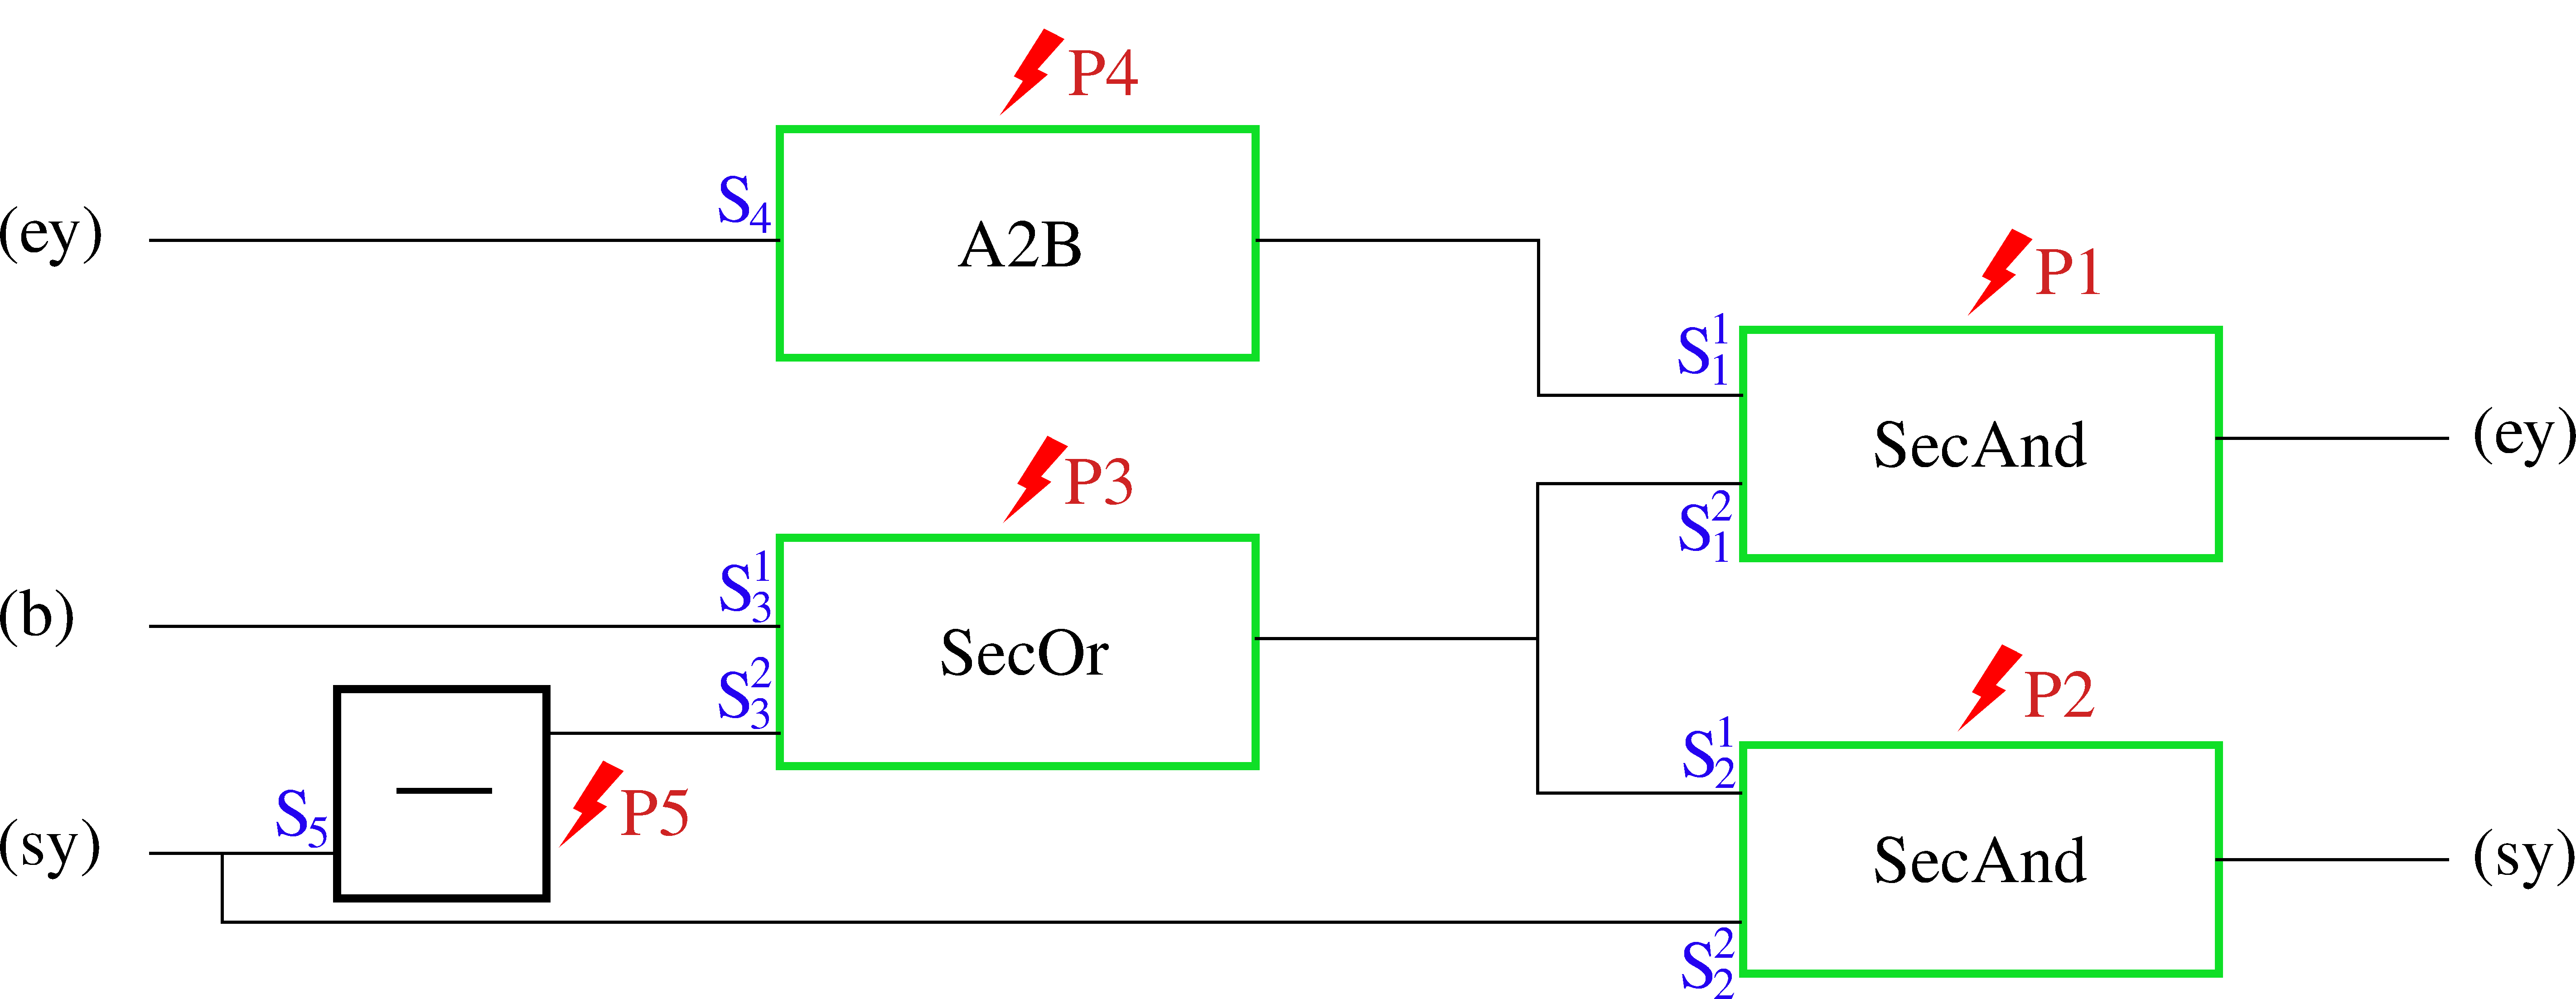
\includegraphics[width=1\textwidth]{figure/SetExZero.pdf}
  \label{fig:SetExponentZero}
  \caption{SetExponentZero}
\end{figure}

\subsection{SecFprUrsh$_\text{floor}$}

FAIRE LA PREUVE

\begin{figure}[h!]
  \centering
  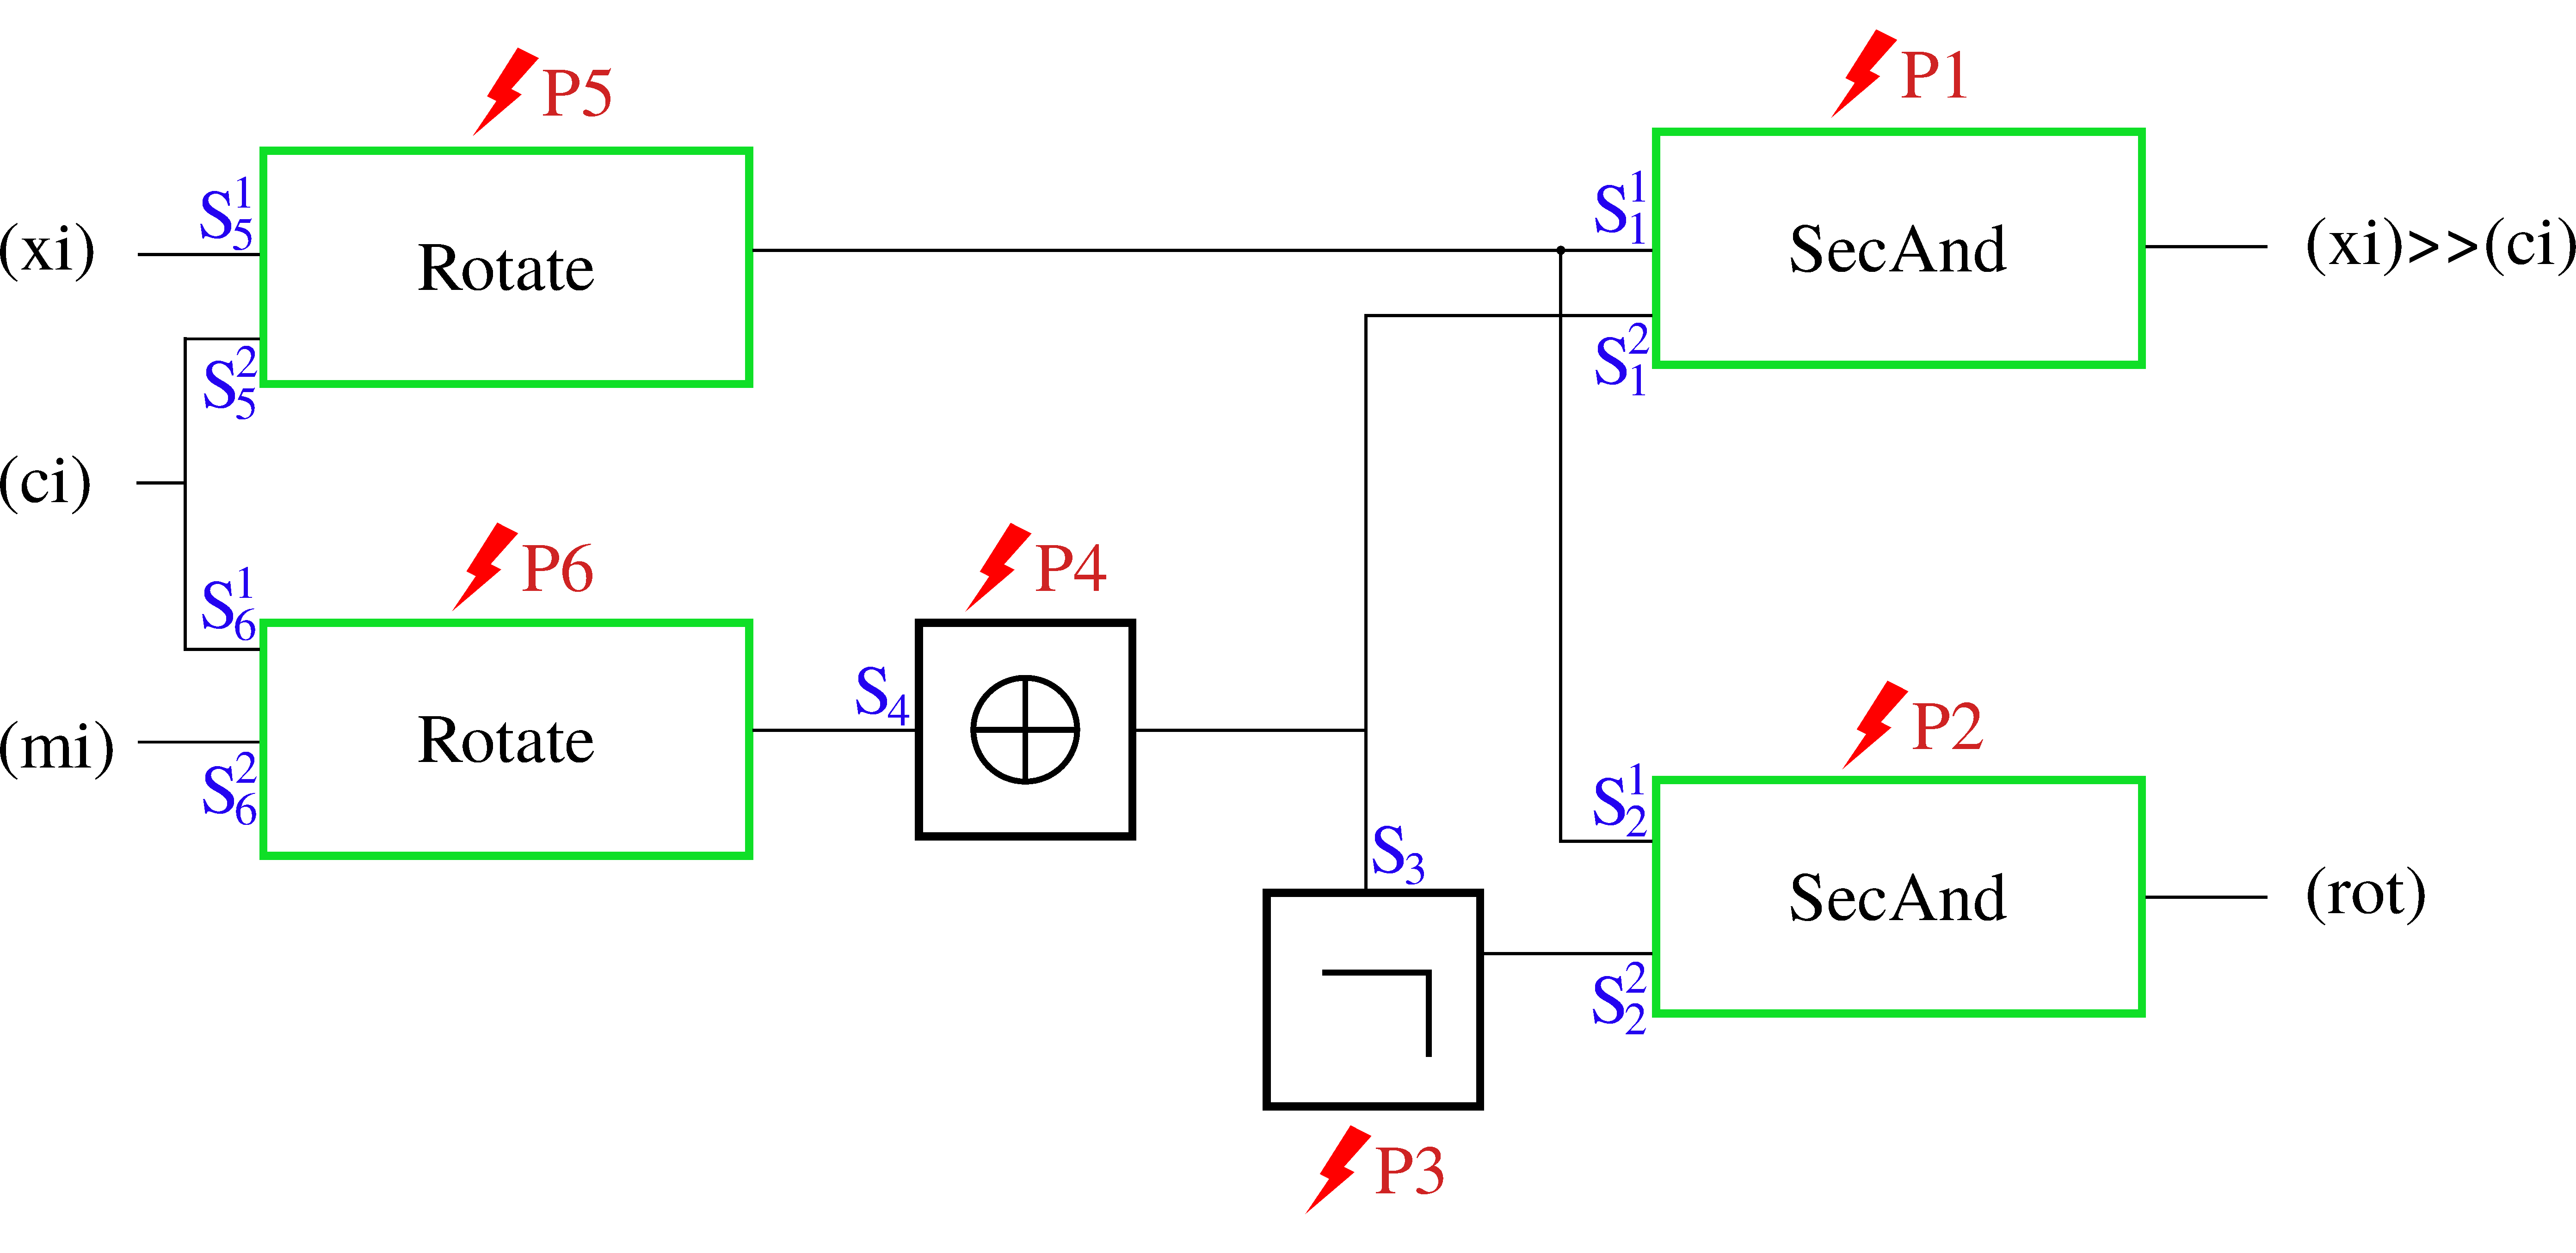
\includegraphics[width=1\textwidth]{figure/secfprurshmod.pdf}
  \label{fig:Secfprursh}
  \caption{SecFprUrsh$_f$}
\end{figure}

\subsection{RemoveDecimal$_\text{floor}$}

FAIRE LA PREUVE

\begin{figure}[h!]
  \centering
  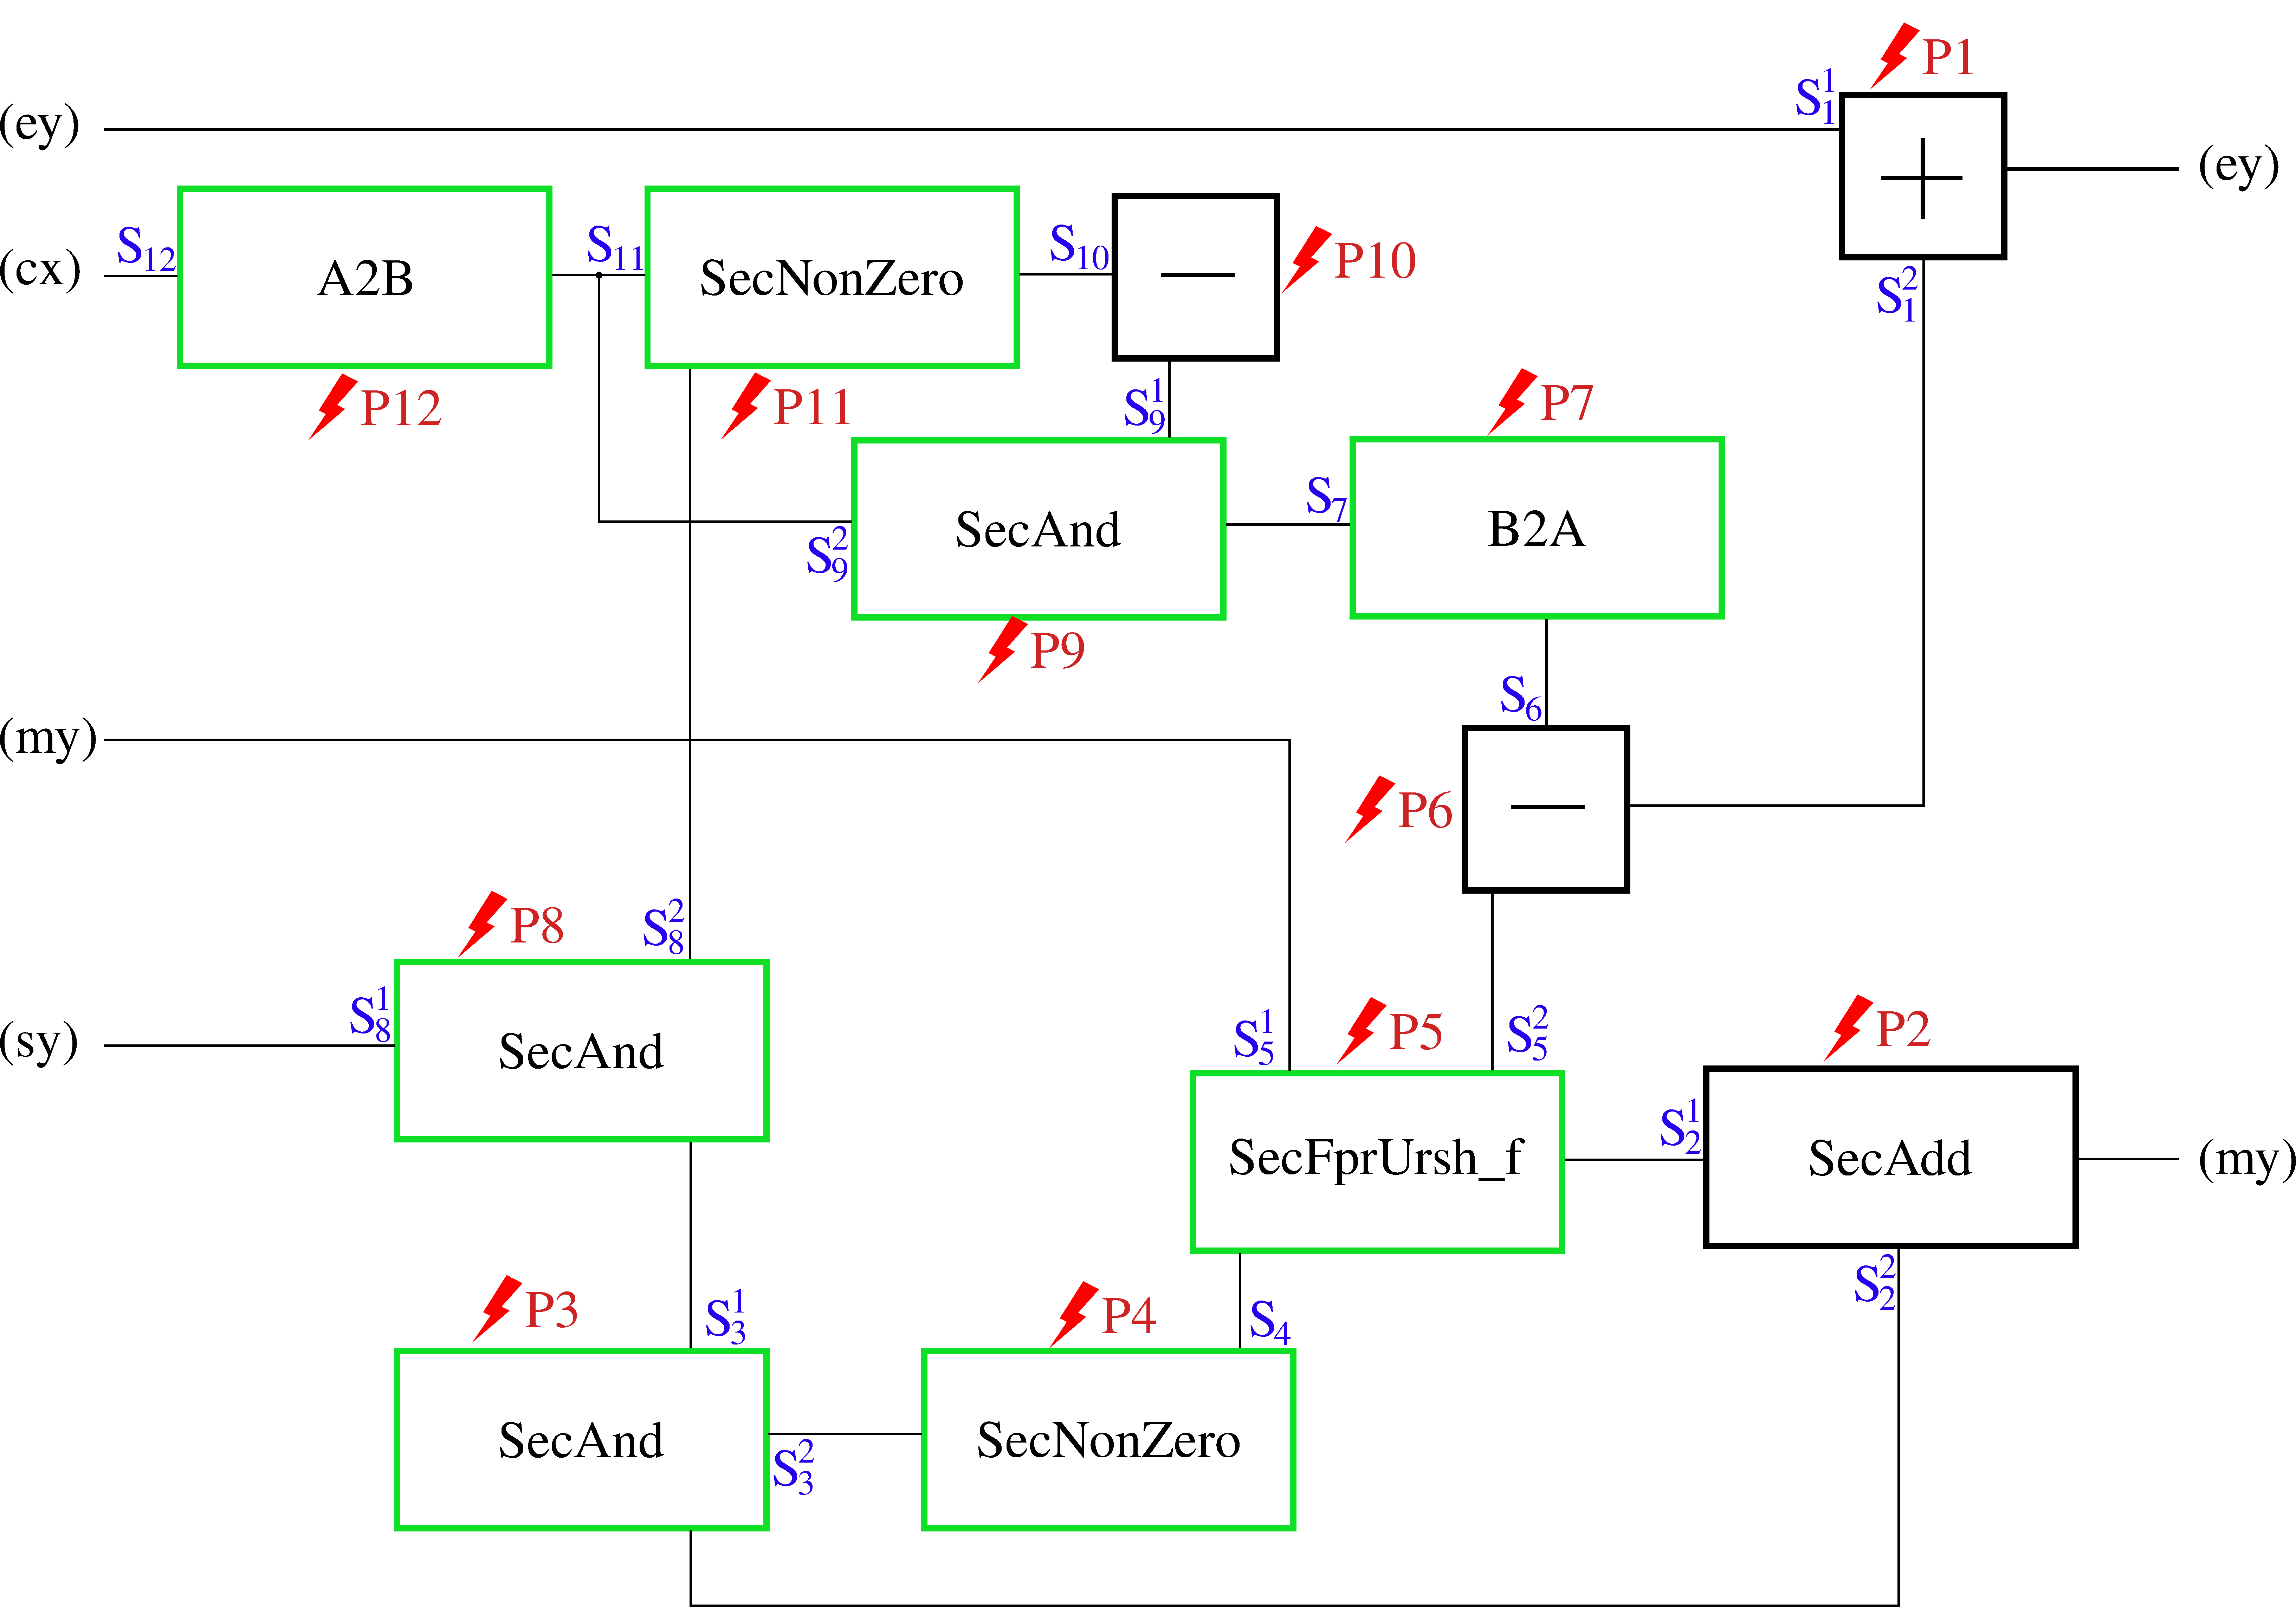
\includegraphics[width=1\textwidth]{figure/RemoveDec.pdf}
  \label{fig:Secfprursh}
  \caption{SecFprUrsh$_f$}
\end{figure}

\subsection{SecBaseInt$_\text{floor}$}

FAIRE LA PREUVE

\begin{figure}[h!]
  \centering
  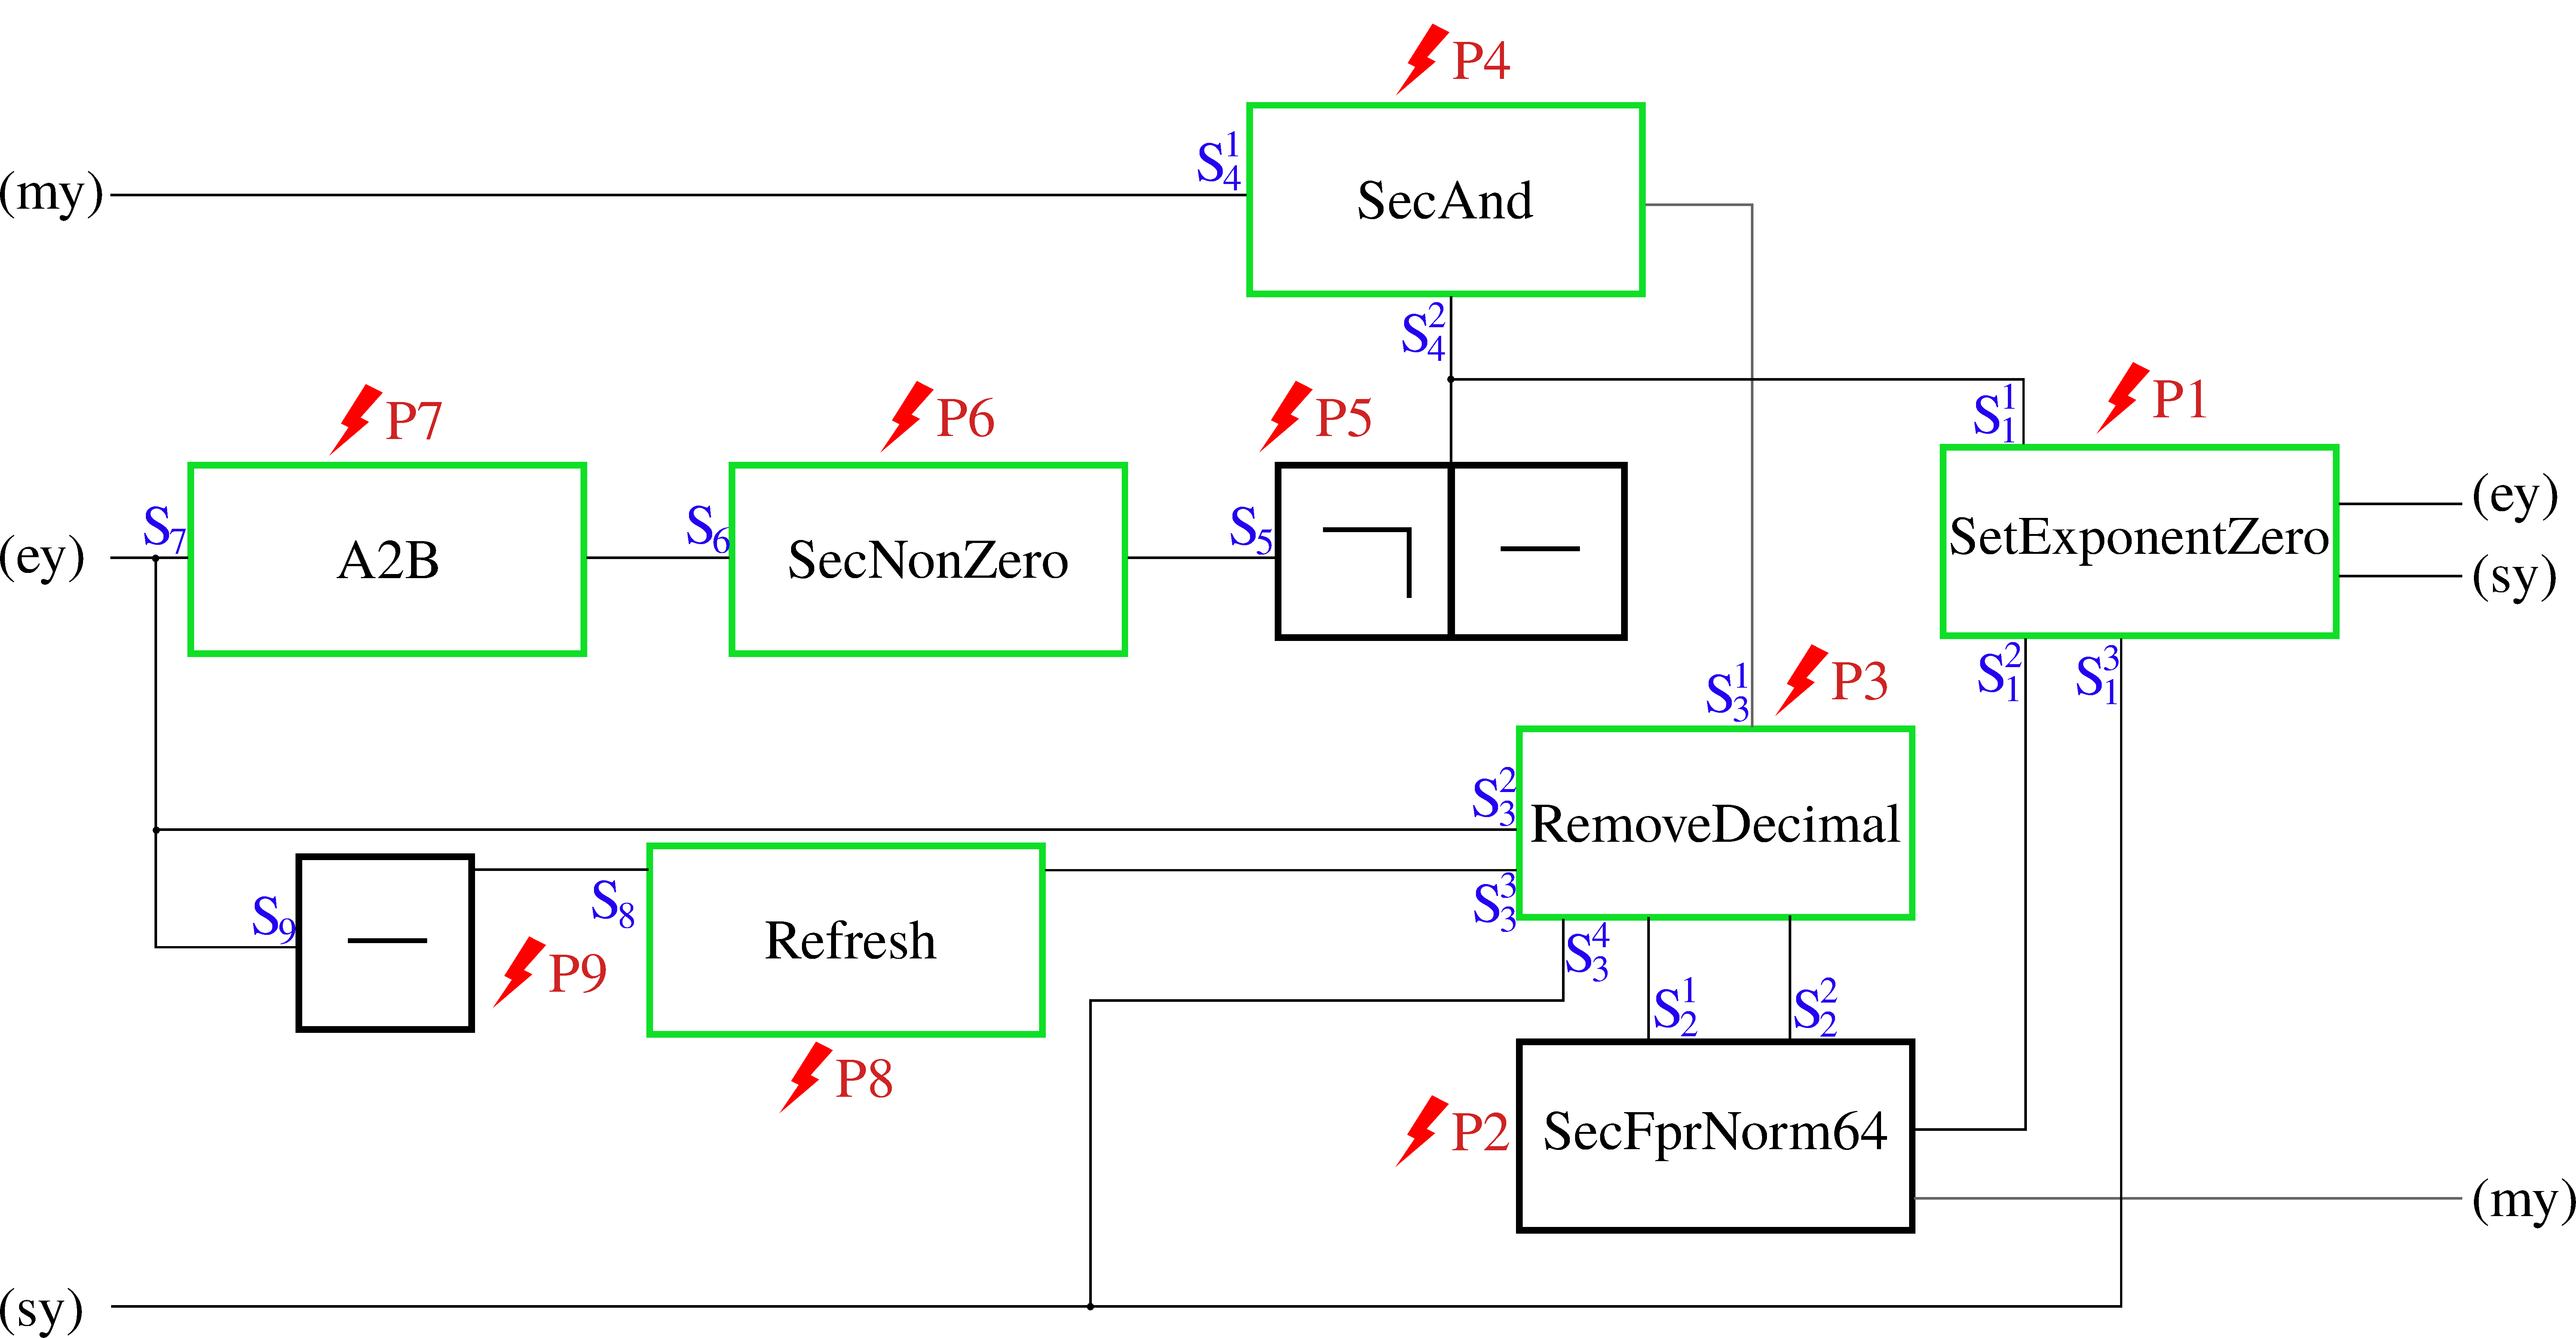
\includegraphics[width=1\textwidth]{figure/secbaseint.pdf}
  \label{fig:Secfprursh}
  \caption{SecFprUrsh$_f$}
\end{figure}
\newpage

\section{Application to FALCON}\label{sec:appfalcon}
\subsection{Masked Floor Function For FALCON}
\subsection{Masking the Gaussian Sampler}
\section{Performances}\label{sec:perf}



\section{Conclusion}\label{sec:conclusion}
\subsubsection{Acknowlegdments}

%
% ---- Bibliography ----
%
% BibTeX users should specify bibliography style 'splncs04'.
% References will then be sorted and formatted in the correct style.
%

\newpage


 \bibliographystyle{splncs04}
 \bibliography{falcon}

\newpage

\section*{Appendix}


\subsection*{Extract}

\begin{algorithm}
  \caption{SecFprExtract(x)}
  \label{algo:SecFprExtract }
  \KwData{64-bit boolean shares $(x_i)_{1\leq i \leq n}$ for value x}
  \KwResult{64-bit boolean shares $(mx_i)_{1\leq i \leq n}$ for mantissa value mx; \\
            16-bit arithmetic shares $(ex_i)_{1\leq i \leq n}$ for exponent value ex; \\
            1-bit boolean shares $(sx_i)_{1\leq i \leq n}$ for sign value s.} 
  $(mx_i) \leftarrow (x_i^{[52:1]})$\;
  $(mx_i) \leftarrow$ SecAdd$((mx_i), (2^{52}, 0, \cdots, 0))$\tcp*{add implicit bit in the mantissa} 
  $(ex_i) \leftarrow (x_i^{[63:53]})$\;
  $(ex_i) \leftarrow$ B2A($(ex_i)$)\;
  $(sx_i) \leftarrow (x_i^{(64)})$\;
\Return{$((mx_i), (ex_i), (sx_i))$}\;
\end{algorithm}

\newpage
\subsection*{Truncature Function: Gadgets}

\begin{algorithm}
  \caption{RemoveDecimal$_{\text{trunc}}((my_i), (ey_i), (sy_i), (cx_i))$}
  \KwData{64-bit boolean shares $(my_i)_{1\leq i \leq n}$ for mantissa value my; \\
  16-bit arithmetic shares $(ey_i)_{1\leq i \leq n}$ for exponent value ey; \\
  1-bit boolean shares $(sy_i)_{1\leq i \leq n}$ for sign value sy\\
  16-bit arithmetic shares $(cx_i)_{1\leq i \leq n}$ for value cx = ex-2013.}
  \KwResult{64-bit boolean shares $(my_i)_{1\leq i \leq n}$ for mantissa value $my >> (52 - cx)$; \\
            16-bit arithmetic shares $(ey_i)_{1\leq i \leq n}$ for exponent value $ey +(52 - cx)$;} 
  $cx_1 \leftarrow cx_1 - 52$\tcp*{check if 0$\leq$c$<$51}
  $(c_i) \leftarrow$ A2B($(cx_i)$)\;
  $(cp_i) \leftarrow (c_i^{(16)})$\;
  $(cp_i) \leftarrow$ SecNonZero($cp_i$)\;
  $(c'_i) \leftarrow (- cp_i)$\tcp*{if cp = 0 cx = 0. if not cx = cx }
  $(c_i) \leftarrow$ SecAnd($(c_i), (cp_i)$)\;
  $(cx_i) \leftarrow$ B2A($(c_i)$)\;
  $(cd_i) \leftarrow (-cx_i)$\;
  $(my_i) \leftarrow$ SecFprUrsh$_f$($(my_i), (cd_i)$)\tcp*{$my >> 52 - cx$}
  $(ey_i) \leftarrow (ey_i + cd_i)$\; 
\Return{$((my_i), (ey_i))$}\;
\end{algorithm}



\begin{algorithm}
  \caption{SetExponentZero$_{\text{trunc}}((ey_i), (sy_i), (b_i))$}
  \KwData{ 16-bit arithmetic shares $(ey_i)_{1\leq i \leq n}$ for exponent value ey; \\
  1-bit boolean shares $(sy_i)_{1\leq i \leq n}$ for sign value sy\\
  64-bit boolean shares $(b_i)_{1\leq i \leq n}$.}
  \KwResult{16-bit boolean shares $(ey_i)_{1\leq i \leq n}$ for exponent value $ey +(52 - cx)$;\\
            1-bit boolean shares $(sy_i)_{1\leq i \leq n}$ for sign value.} 
  
    $(ey_i) \leftarrow$ A2B($(ey_i)$)\;
    %$(b'_i) \leftarrow (-sy_i)$\;
    $(ey_i) \leftarrow$ SecAnd($(ey_i, b_i)$)\;
    $(sy_i) \leftarrow$ SecAnd($(sy_i, b_i)$)\;

\Return{$((ey_i), (sy_i))$}\;
\end{algorithm}



\newpage
\subsection*{Round Function: Gadgets}

\begin{algorithm}
  \caption{RemoveDecimal$_{\text{round}}((my_i), (ey_i), (sy_i), (cx_i))$}
  \KwData{64-bit boolean shares $(my_i)_{1\leq i \leq n}$ for mantissa value my; \\
  16-bit arithmetic shares $(ey_i)_{1\leq i \leq n}$ for exponent value ey; \\
  1-bit boolean shares $(sy_i)_{1\leq i \leq n}$ for sign value sy\\
  16-bit arithmetic shares $(cx_i)_{1\leq i \leq n}$ for value cx = ex-2013.}
  \KwResult{64-bit boolean shares $(my_i)_{1\leq i \leq n}$ for mantissa value $my >> (52 - cx)$; \\
            16-bit arithmetic shares $(ey_i)_{1\leq i \leq n}$ for exponent value $ey +(52 - cx)$;\\
            1-bit boolean shares $(Rnd_i)$ for value Rnd -- the bit at position -1.} 
  $cx_1 \leftarrow cx_1 - 53$\tcp*{check if 0$\leq$c$<$51}
  $(c_i) \leftarrow$ A2B($(cx_i)$)\;
  $(cp_i) \leftarrow (c_i^{(16)})$\;
  $(cp_i) \leftarrow$ SecNonZero($cp_i$)\;
  $(rshORnot_i) \leftarrow (-cp[i])$\; 
  $(c'_i) \leftarrow (- cp_i)$\tcp*{if cp = 0 cx = 0. if not cx = cx }
  $cx_1 \leftarrow cx_1 + 1$\;
  $(c_i) \leftarrow$ A2B($(cx_i)$)\;
  $(c_i) \leftarrow$ SecAnd($(c_i), (cp_i)$)\;
  $(cx_i) \leftarrow$ B2A($(c_i)$)\;
  $(cd_i) \leftarrow (-cx_i)$\;
  $(my_i) \leftarrow$ SecFprUrsh($(my_i), (cd_i)$)\tcp*{$my >> 53 - cx$}
  $(Rnd_i) \leftarrow (my_i^{(1)})$\;
  $(Rnd_i) \leftarrow$ SecNonZero$(Rnd_i)$\;
  $(Rnd_i) \leftarrow$ SecAnd($(Rnd_i), (rshORnot_i)$)\;
  $(my1_i) \leftarrow$ $(my_i)>>1$ , $\quad (e1_i) \leftarrow$ $(1,0,\cdots, 0)$\;
  $(my2_i) \leftarrow$ $(my_i)\qquad \quad$,  $\quad(e2_i) \leftarrow$ $(0,\cdots, 0)$\;
  $(my1_i) \leftarrow$ SecAnd($(my1_i), (rshORnot_i))\quad $, $(e1_i) \leftarrow$ SecAnd($(e1_i), (rshORnot_i)$)\;
  $(rshORnot_i) \leftarrow (-rshORnot_i)$\;
  $(my2_i) \leftarrow$ SecAnd($(my2_i), (rshORnot_i))\quad $, $(e2_i) \leftarrow$ SecAnd($(e2_i), (rshORnot_i)$)\;
  $(my_i) \leftarrow$ SecOr($(my1_i), (my2_i)$)\;
  $(my_i) \leftarrow$ SecAdd($(my_i), (Rnd_i)$)\;
  $(e1_i) \leftarrow$ SecOr($(e1_i), (e2_i)$)\;
  $(e1_i) \leftarrow$ B2A($(e1_i)$)\; 
  $(ey_i) \leftarrow (ey_i + e1_i) $\;
  $(ey_i) \leftarrow (ey_i + cd_i)$\; 
\Return{$((my_i), (ey_i), (Rnd_i))$}\;
\end{algorithm}

\begin{algorithm}
  \caption{SetExponentZero$_{\text{round}}((ey_i), (sy_i), (b_i), (Rnd_i))$}
  \KwData{ 16-bit arithmetic shares $(ey_i)_{1\leq i \leq n}$ for exponent value ey; \\
  1-bit boolean shares $(sy_i)_{1\leq i \leq n}$ for sign value sy\\
  64-bit boolean shares $(b_i)_{1\leq i \leq n}$.}
  \KwResult{16-bit boolean shares $(ey_i)_{1\leq i \leq n}$ for exponent value $ey +(52 - cx)$;\\
            1-bit boolean shares $(sy_i)_{1\leq i \leq n}$ for sign value.} 
  
    $(ey_i) \leftarrow$ A2B($(ey_i)$)\;
    $(b'_i) \leftarrow (Rnd_i)$\;
    $(b'_i) \leftarrow$ SecOr($(b'_i), (b_i)$)\;
    $(ey_i) \leftarrow$ SecAnd($(ey_i, b'_i)$)\;
    $(sy_i) \leftarrow$ SecAnd($(sy_i, b'_i)$)\;

\Return{$((ey_i), (sy_i))$}\;
\end{algorithm}

\end{document}
